\documentclass[10pt, reqno]{article}		% sets document class
\usepackage[usenames,dvipsnames]{pstricks}
\usepackage{epsfig}
\usepackage{pst-grad} 				% enables gradients
\usepackage{pst-plot} 				% enables axes
\usepackage[space]{grffile} 		% enables spaces in paths
\usepackage{etoolbox} 				% enables spaces in paths
\makeatletter 						% enables spaces in paths
\patchcmd\Gread@eps{\@inputcheck#1 }{\@inputcheck"#1"\relax}{}{}
\makeatother
\usepackage[margin=1.0in]{geometry}	% sets paper size
\usepackage{amssymb}				% enables formulas
\usepackage{amsmath}				% enables formulas
\usepackage[utf8]{inputenc}			% enables diacritical input
\usepackage{graphicx}				% enables graphics
\graphicspath{ {images/} }			% sets graphics path
\usepackage{chngcntr}				% enables counter
\counterwithin{table}{subsection}	% enables table pre-labels
\counterwithin{figure}{subsection}	% enables figure pre-labels
\usepackage[labelsep=endash, labelfont=bf, font=bf]{caption}	% sets figure and caption separator
%\usepackage{indentfirst}			% enables indent on first paragraphs
\linespread{1.1}					% sets spacing to 1.5
\setlength{\parskip}{0.5em}			% sets paragraph spacing to 1m
%\usepackage{times}					% sets font to times new roman
\usepackage{wrapfig}				% enables text wrapping around figures
\usepackage{gensymb}				% enables symbols
\usepackage{endnotes}				% enables endnotes
\usepackage{afterpage}				% enables afterpage capability
\setcounter{secnumdepth}{3}			% sets counter recognitions to sssection for label capability
\numberwithin{equation}{section}
\makeatletter						% set figure labels to center
\g@addto@macro\@floatboxreset\centering
\makeatother
\usepackage{setspace}				% enables environments for spacing
\usepackage{graphicx}				% allows table usage
\usepackage{hyperref}				% enables hyperlinks
\hypersetup{colorlinks=false, linkcolor=cyan, urlcolor=cyan, linktoc=page} % sets hyperlink colors
\usepackage{accents}				% enables accents
\usepackage{textcomp} 				% enables copyright
\usepackage{tabto}					% enables tabbing
\setlength\parindent{0pt}			% sets no indents
\usepackage[framed]{mcode} 			% enables code boxes
\usepackage{titlesec}				% enables title formatting
\titleformat{\part}{\filcenter\huge\bfseries}{}{}{}
\usepackage{float}

\begin{document}

\newcommand{\stoptocwriting}{%
	\addtocontents{toc}{\protect\setcounter{tocdepth}{-5}}}
\newcommand{\resumetocwriting}{%
	\addtocontents{toc}{\protect\setcounter{tocdepth}{\arabic{tocdepth}}}}

\stoptocwriting
\part*{\underline{AERO 430 -- Numerical Simulation} \\ \Large Second-Order Linear Ordinary Differential Equation Boundary-Value Problem for 1-D Convection-Diffusion Equation \\ \large Ross B. Alexander}
\resumetocwriting

\vfill

\begin{figure}[h]
	\begin{center}
	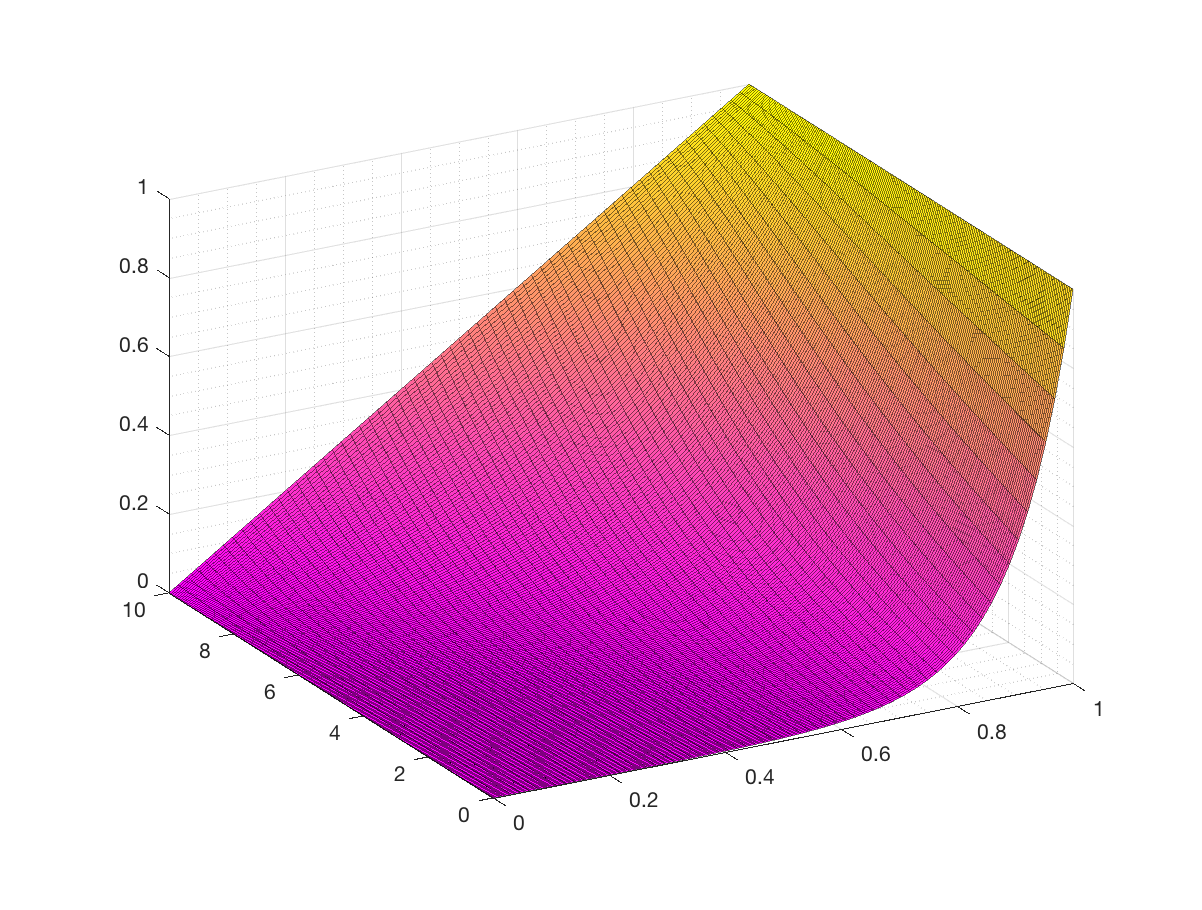
\includegraphics[width = 0.98\linewidth]{title_image}
	\end{center}
\end{figure}

\vspace{80pt}

\newpage

\tableofcontents

\newpage

\section{Model Problem}

The model second-order linear ordinary differential equation boundary-value problem consists of:
\begin{itemize}
	\item the second-order linear ordinary differential equation:
	\begin{equation}
	- u''(x)+cu'(x)=0 \qquad x \in (0, 1)
	\end{equation}
	\item the boundary conditions:
	\begin{equation}
	u(0) = 0 \quad \textnormal{and} \quad u(1) = 1 
	\end{equation}
\end{itemize}
The physical model of the second-order linear ordinary differential equation boundary-value problem is that of the concentration of a flow property that convects and diffuses proportional to the constant $c$. For example, the convection-diffusion equation could represent the concentration of ink as a function of distance in a quasi-one-dimensional flow.

\newpage

\section{Analytical Solution}

\subsection{Analytical Solution to the Differential Equation}

The following equation is the homogeneous second-order linear ordinary differential equation (ODE).
\begin{equation}
- u''(x)+cu'(x)=0
\end{equation}
The solution of the homogeneous ODE, $u_h(x)$ is assumed to be of the form: 
\begin{equation}
u_h(x) = e^{\lambda x}
\end{equation}
Taking the derivatives of $u_h(x)$, substituting them into the homogeneous ODE, and reducing the equation yields the \textbf{characteristic equation}.
\begin{equation}
u'_h(x) = \lambda e^{\lambda x}
\end{equation}
\begin{equation}
u''_h(x) = \lambda^2 e^{\lambda x}
\end{equation}
\begin{equation}
-\lambda^2 e^{\lambda x} + c \lambda e^{\lambda x} = 0
\end{equation}
\begin{equation}
\mathbf{-\lambda^2 + c \lambda = \lambda(c-\lambda) = 0}
\end{equation}
Solving for $\lambda$ yields:
\begin{equation}
\lambda = \{0, c\}
\end{equation}
The homogenous solution $u_h(x)$ is then:
\begin{equation}
u_h(x) = ae^{0x} + be^{cx} 
\end{equation}
\begin{equation}
\mathbf{u_h(x) = a + be^{cx}}
\end{equation}
Applying the both boundary conditions, $u(0) = 0$ and $u(1) = 1$, we get the system of algebraic equations, which yields $a$ and $b$:
\begin{equation}
u_h(0) = 0 = a + b
\end{equation}
\begin{equation}
u_h(1) = 1 = a + be^c
\end{equation}
\begin{equation}
	\begin{bmatrix}
		1 & 1 \\ 1 & e^c
	\end{bmatrix}
	\begin{bmatrix}
	a \\ b
	\end{bmatrix}
	=
	\begin{bmatrix}
	0 \\ 1
	\end{bmatrix}
\end{equation}
\begin{equation}
a = \frac{-1}{e^c-1} \quad \textnormal{and} \quad b = \frac{1}{e^c-1}
\end{equation}
Thus, it is shown that for the second-order linear ordinary differential equation with specified boundary conditions, that $u(x)$ is a solution to the differential equation on $x \in (0, 1)$.
\begin{equation}
-u''(x)+cu'(x)=0 \qquad x \in (0, 1)
\end{equation}
\begin{equation}
u(0) = 0 \quad \textnormal{and} \quad u(1) = 1 
\end{equation}
\begin{equation}
\mathbf{u(x) = \frac{e^{cx}-1}{e^c-1}}
\end{equation}

\newpage

The values of $c$ tested in this study were $c \in {1, 2, 5, 10, 20, 50}$. A plot of the analytical solution for values of $c$ is depicted below:
\begin{figure}[H]
	\begin{center}
		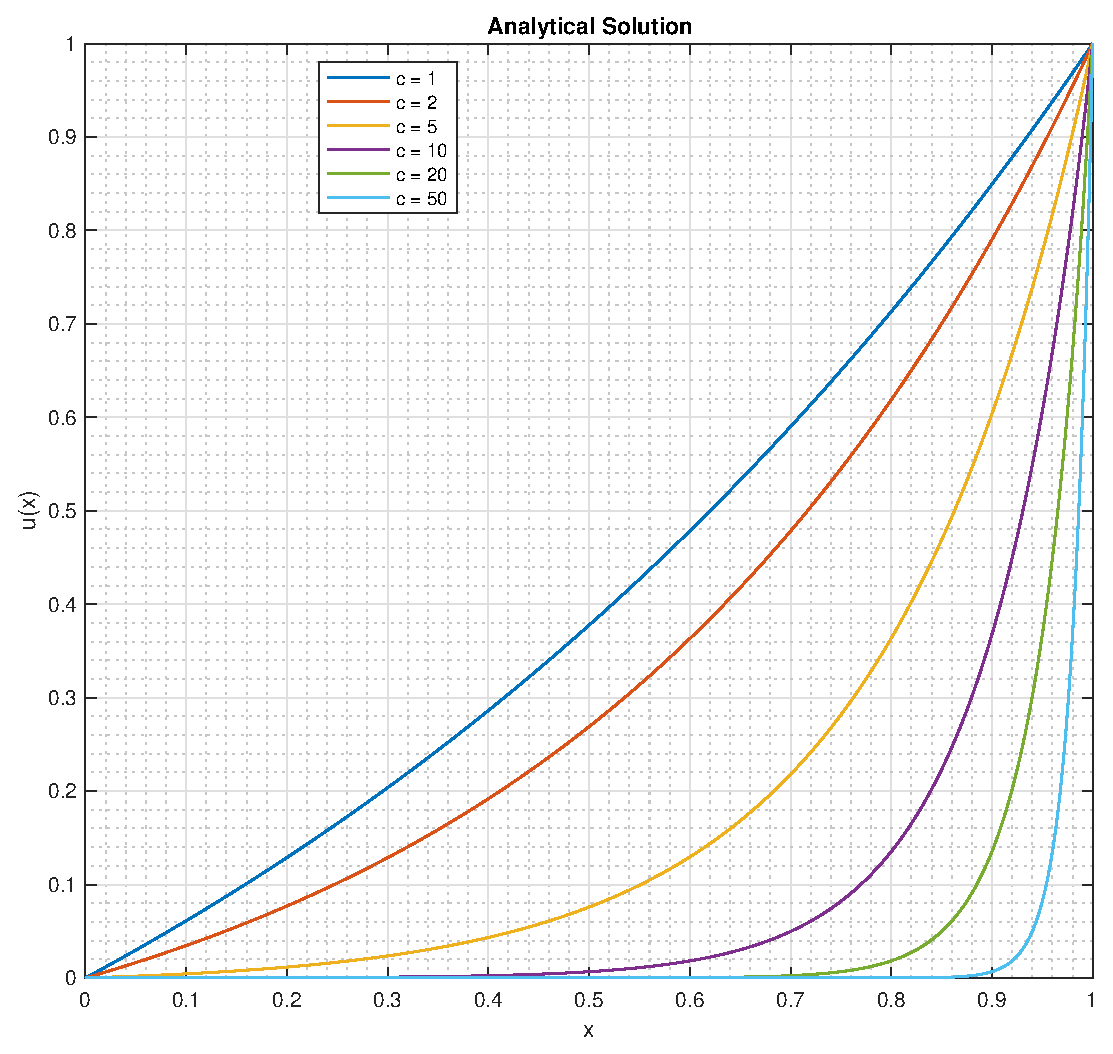
\includegraphics[width = 0.8\linewidth]{analytical_solution}
		\caption{Analytical Solution to the Differential Equation for Values of $c$}
	\end{center}
\end{figure}

\newpage

\subsection{Analytical Solution to the Quantity of Interest}

The quantity of interest for this particular problem is the first derivative at the right boundary, or $u'(1)$. The differential equation and the analytical solution to the differential equation, respectively, are reproduced below.
\begin{equation}
- u''(x)+cu'(x)=0
\end{equation}
\begin{equation}
u(x) = \frac{e^{cx}-1}{e^c-1}
\end{equation}
Thus, taking the first derivative, and solving at $x = 1$, we obtain the exact quantity of interest:
\begin{equation}
u'(x) = \frac{ce^{cx}}{e^c-1}
\end{equation}
\begin{equation}
\mathbf{u'(1) = \frac{ce^{c}}{e^c-1}}
\end{equation}
It can be seen that if $e^c$, or rather $c$, is sufficiently large ($e^c \gg 1$), then the quantity of interest tends to $c$ given that the ratio of $e^c$ and $(e^c -1)$ tends to unity:
\begin{equation}
\lim_{c\to\infty} \frac{ce^{c}}{e^c-1} = \infty \approxeq c
\end{equation}

A table of the exact quantity of interest for the tested values of $c$ is included below (for $c=50$, error is less than machine epsilon, $\epsilon$):
\begin{table}[H]
	\caption{Analytical Solution to the Quantity of Interest for Values of $c$}
\begin{tabular}{|c|c|}
	\hline 
	$\mathbf{c}$ & $\mathbf{u'(1)}$ \\ 
	\hline 
	1 & 1.58198 \\ 
	\hline 
	2 & 2.31304 \\ 
	\hline 
	5 & 5.03392 \\ 
	\hline 
	10 & 10.00045 \\ 
	\hline 
	20 & 20.00000004 \\ 
	\hline 
	50 & 50.00000000 \\ 
	\hline 
\end{tabular}
\end{table} 

\newpage

\section{Numerical Methods}

\subsection{Derivations}

\subsubsection{2nd-Order Central Difference Scheme Finite Difference Method}

\paragraph{First Derivative}
Developing the Taylor series for $u(x)$ in the vicinity of $x = i$:
\begin{equation}
u_{i-1} = u_i - \Delta x u'_i + \frac{\Delta x^2}{2} u''_i - \frac{\Delta x^3}{6} u^{(3)}_i + \frac{\Delta x^4}{24} u^{(4)}_i + \mathcal{O}(\Delta x^5)
\end{equation}
\begin{equation}
u_{i+1} = u_i + \Delta x u'_i + \frac{\Delta x^2}{2} u''_i + \frac{\Delta x^3}{6} u^{(3)}_i + \frac{\Delta x^4}{24} u^{(4)}_i + \mathcal{O}(\Delta x^5)
\end{equation}
Subtracting the Taylor series for $u_{i-1}$ from $u_{i+1}$ and canceling terms:
\begin{equation}
u_{i+1} - u_{i-1} = 2\Delta xu'_i + \frac{\Delta x^3}{3} u^{(3)}_i + \mathcal{O}(\Delta x^5)
\end{equation}
Solving for $u'_i$:
\begin{equation}
u'_i = \frac{u_{i+1} - u_{i-1}}{2 \Delta x} + \mathcal{O}(\Delta x^2) 
\end{equation}

From this specific first-derivative formulation using the finite difference method, the first-derivative approximation can be observed to be second-order ($\mathcal{O}(\Delta x^2)$).

\paragraph{Second Derivative}
Developing the Taylor series for $u(x)$ in the vicinity of $x = i$:
\begin{equation}
u_{i-1} = u_i - \Delta x u'_i + \frac{\Delta x^2}{2} u''_i - \frac{\Delta x^3}{6} u^{(3)}_i + \frac{\Delta x^4}{24} u^{(4)}_i + \mathcal{O}(\Delta x^5)
\end{equation}
\begin{equation}
u_{i+1} = u_i + \Delta x u'_i + \frac{\Delta x^2}{2} u''_i + \frac{\Delta x^3}{6} u^{(3)}_i + \frac{\Delta x^4}{24} u^{(4)}_i + \mathcal{O}(\Delta x^5)
\end{equation}
Adding the Taylor series for $u_{i-1}$ and $u_{i+1}$ and canceling terms:
\begin{equation}
u_{i+1} + u_{i-1} = 2u_i + \Delta x^2 u''_i + \mathcal{O}(\Delta x^4)
\end{equation}
Rearranging terms to solve for $u''_i$:
\begin{equation}
u''_i = \frac{u_{i+1} - 2u_i + u_{i-1}}{\Delta x^2} + \mathcal{O}(\Delta x^2) 
\end{equation}

From this specific second-derivative formulation using the finite difference method, the second-derivative approximation can be observed to be second-order ($\mathcal{O}(\Delta x^2)$).

\paragraph{Discretized Differential Equation}
The differential equation is:
\begin{equation}
- u''(x)+cu'(x)=0
\end{equation}
Discretizing using the above formulas and simplifying yields:
\begin{equation}
-\left(\frac{u_{i+1} - 2u_i + u_{i-1}}{\Delta x^2}\right) + c\left(\frac{u_{i+1} - u_{i-1}}{2 \Delta x}\right) = 0
\end{equation}
\begin{equation}
-\left(u_{i+1} - 2u_i + u_{i-1}\right) + c\Delta x\left( \frac{u_{i+1} - u_{i-1}}{2}\right) = 0
\end{equation}
\begin{equation}
\left(-1-\frac{c\Delta x}{2}\right)u_{i-1} + \left(2\right)u_{i} + \left(-1+\frac{c\Delta x}{2}\right)u_{i+1} = 0
\end{equation}

\subsubsection{4th-Order Central Difference Scheme Finite Difference Method}

\paragraph{First Derivative}
Developing the Taylor series for $u(x)$ in the vicinity of $x = i$:
\begin{equation}
u_{i-1} = u_i - \Delta x u'_i + \frac{\Delta x^2}{2} u''_i - \frac{\Delta x^3}{6} u^{(3)}_i + \frac{\Delta x^4}{24} u^{(4)}_i + \mathcal{O}(\Delta x^5)
\end{equation}
\begin{equation}
u_{i+1} = u_i + \Delta x u'_i + \frac{\Delta x^2}{2} u''_i + \frac{\Delta x^3}{6} u^{(3)}_i + \frac{\Delta x^4}{24} u^{(4)}_i + \mathcal{O}(\Delta x^5)
\end{equation}
Subtracting the Taylor series for $u_{i-1}$ from $u_{i+1}$ and canceling terms:
\begin{equation}
u_{i+1} - u_{i-1} = 2\Delta xu'_i + \frac{\Delta x^3}{3} u^{(3)}_i + \mathcal{O}(\Delta x^5)
\end{equation}
Returning to the differential equation and taking one additional derivative:
\begin{equation}
u''(x)=cu'(x)
\end{equation}
\begin{equation}
u^{(3)}(x)=cu''(x)
\end{equation}
Replacing the second-derivative term with the original differential equation:
\begin{equation}
u^{(3)}(x) = c^2u'(x)
\end{equation}
Now replacing the third-derivative term in the Taylor series subtraction and then dividing by $2\Delta x$:
\begin{equation}
u_{i+1} - u_{i-1} = 2\Delta xu'_i + \frac{c^2\Delta x^3}{3}u'_i  + \mathcal{O}(\Delta x^5)
\end{equation}
\begin{equation}
\frac{u_{i+1} - u_{i-1}}{2\Delta x} = \left(1 + \frac{c^2\Delta x^2}{6}\right)u'_i  + \mathcal{O}(\Delta x^4)
\end{equation}
Solving for $u'_i$:
\begin{equation}
u'_i = \left(1 + \frac{c^2\Delta x^2}{6}\right)^{-1} \frac{u_{i+1} - u_{i-1}}{2\Delta x} + \mathcal{O}(\Delta x^4)
\end{equation}

From this specific first-derivative formulation using the finite difference method, the first-derivative approximation can be observed to be fourth-order ($\mathcal{O}(\Delta x^4)$).

\paragraph{Second Derivative}
Developing the Taylor series for $u(x)$ in the vicinity of $x = i$:
\begin{equation}
u_{i-1} = u_i - \Delta x u'_i + \frac{\Delta x^2}{2} u''_i - \frac{\Delta x^3}{6} u^{(3)}_i + \frac{\Delta x^4}{24} u^{(4)}_i + \mathcal{O}(\Delta x^5)
\end{equation}
\begin{equation}
u_{i+1} = u_i + \Delta x u'_i + \frac{\Delta x^2}{2} u''_i + \frac{\Delta x^3}{6} u^{(3)}_i + \frac{\Delta x^4}{24} u^{(4)}_i + \mathcal{O}(\Delta x^5)
\end{equation}
Adding the Taylor series for $u_{i-1}$ and $u_{i+1}$ and canceling terms:
\begin{equation}
u_{i+1} + u_{i-1} = 2u_i + \Delta x^2 u''_i + \frac{\Delta x^4}{12} u^{(4)}_i + \mathcal{O}(\Delta x^6)
\end{equation}
Returning to the differential equation and taking two additional derivatives:
\begin{equation}
u''(x)=cu'(x)
\end{equation}
\begin{equation}
u^{(3)}(x)=cu''(x)
\end{equation}
\begin{equation}
u^{(4)}(x)=cu^{(3)}(x)
\end{equation}
Replacing the fourth-derivative and third-derivative terms with the original differential equation, we arrive at:
\begin{equation}
u^{(4)}(x) = c^2u''(x)
\end{equation}
Now replacing the fourth-derivative term in the Taylor series addition, rearranging, and dividing by $\Delta x^2$:
\begin{equation}
u_{i+1} + u_{i-1} = 2u_i + \Delta x^2 u''_i + \frac{c^2\Delta x^4}{12} u''_i + \mathcal{O}(\Delta x^6)
\end{equation}
\begin{equation}
\frac{u_{i+1} -2u_i + u_{i-1}}{\Delta x^2} =  \left(1 + \frac{c^2\Delta x^2}{12} \right)u''_i + \mathcal{O}(\Delta x^4)
\end{equation}
Rearranging terms to solve for $u''_i$:
\begin{equation}
u''_i = \left(1 + \frac{c^2\Delta x^2}{12} \right)^{-1} \frac{u_{i+1} -2u_i + u_{i-1}}{\Delta x^2} + \mathcal{O}(\Delta x^4)
\end{equation}

From this specific second-derivative formulation using the finite difference method, the second-derivative approximation can be observed to be fourth-order ($\mathcal{O}(\Delta x^4)$).

\paragraph{Discretized Differential Equation}
The differential equation is:
\begin{equation}
- u''(x)+cu'(x)=0
\end{equation}
Discretizing using the above formulas and simplifying yields:
\begin{equation}
-\left(1 + \frac{c^2\Delta x^2}{12} \right)^{-1} \frac{u_{i+1} -2u_i + u_{i-1}}{\Delta x^2} + c\left(1 + \frac{c^2\Delta x^2}{6}\right)^{-1} \frac{u_{i+1} - u_{i-1}}{2\Delta x} = 0
\end{equation}
\begin{equation}
\left(-1-\frac{c\Delta x}{2}-\frac{c^2\Delta x^2}{12}\right)u_{i-1} + \left(2+\frac{c^2\Delta x^2}{6}\right)u_{i} + \left(-1+\frac{c\Delta x}{2}-\frac{c^2\Delta x^2}{12}\right)u_{i+1} = 0
\end{equation}

\subsubsection{1st-Order Upwind Scheme Finite Difference Method}

\paragraph{First Derivative}
Developing the Taylor series for $u(x)$ in the vicinity of $x = i-1$:
\begin{equation}
u_{i-1} = u_i - \Delta x u'_i + \frac{\Delta x^2}{2} u''_i - \frac{\Delta x^3}{6} u^{(3)}_i + \frac{\Delta x^4}{24} u^{(4)}_i + \mathcal{O}(\Delta x^5)
\end{equation}
Rearranging the Taylor series for $u'_i$:
\begin{equation}
u'_i = \frac{u_i - u_{i-1}}{\Delta x}  + \mathcal{O}(\Delta x)
\end{equation}

From this specific first-derivative formulation using the finite difference method, the first-derivative approximation can be observed to be first-order ($\mathcal{O}(\Delta x)$).

\paragraph{Second Derivative}
Developing the Taylor series for $u(x)$ in the vicinity of $x = i$:
\begin{equation}
u_{i-1} = u_i - \Delta x u'_i + \frac{\Delta x^2}{2} u''_i - \frac{\Delta x^3}{6} u^{(3)}_i + \frac{\Delta x^4}{24} u^{(4)}_i + \mathcal{O}(\Delta x^5)
\end{equation}
\begin{equation}
u_{i+1} = u_i + \Delta x u'_i + \frac{\Delta x^2}{2} u''_i + \frac{\Delta x^3}{6} u^{(3)}_i + \frac{\Delta x^4}{24} u^{(4)}_i + \mathcal{O}(\Delta x^5)
\end{equation}
Adding the Taylor series for $u_{i-1}$ and $u_{i+1}$ and canceling terms:
\begin{equation}
u_{i+1} + u_{i-1} = 2u_i + \Delta x^2 u''_i + \mathcal{O}(\Delta x^4)
\end{equation}
Rearranging terms to solve for $u''_i$:
\begin{equation}
u''_i = \frac{u_{i+1} - 2u_i + u_{i-1}}{\Delta x^2} + \mathcal{O}(\Delta x^2) 
\end{equation}

From this specific second-derivative formulation using the finite difference method, the second-derivative approximation can be observed to be second-order ($\mathcal{O}(\Delta x^2)$).

\paragraph{Discretized Differential Equation}
The differential equation is:
\begin{equation}
- u''(x)+cu'(x)=0
\end{equation}
Discretizing using the above formulas and simplifying yields:
\begin{equation}
-\left(\frac{u_{i+1} - 2u_i + u_{i-1}}{\Delta x^2}\right) + c\left(\frac{u_i - u_{i-1}}{\Delta x}\right) = 0
\end{equation}
\begin{equation}
-\left(u_{i+1} - 2u_i + u_{i-1}\right) + c\Delta x\left(u_i - u_{i-1}\right) = 0
\end{equation}
\begin{equation}
\left(-1-c\Delta x\right)u_{i-1} + \left(2+c\Delta x\right)u_{i} + \left(-1\right)u_{i+1} = 0
\end{equation}

\newpage

\subsection{Finite Difference Method Results}

\subsubsection{2nd-Order Central Difference Scheme Finite Difference Method}

\begin{figure}[H]
	\begin{center}
		\includegraphics[width = 0.49\linewidth]{solution_2nd_order_cds_c_1}
		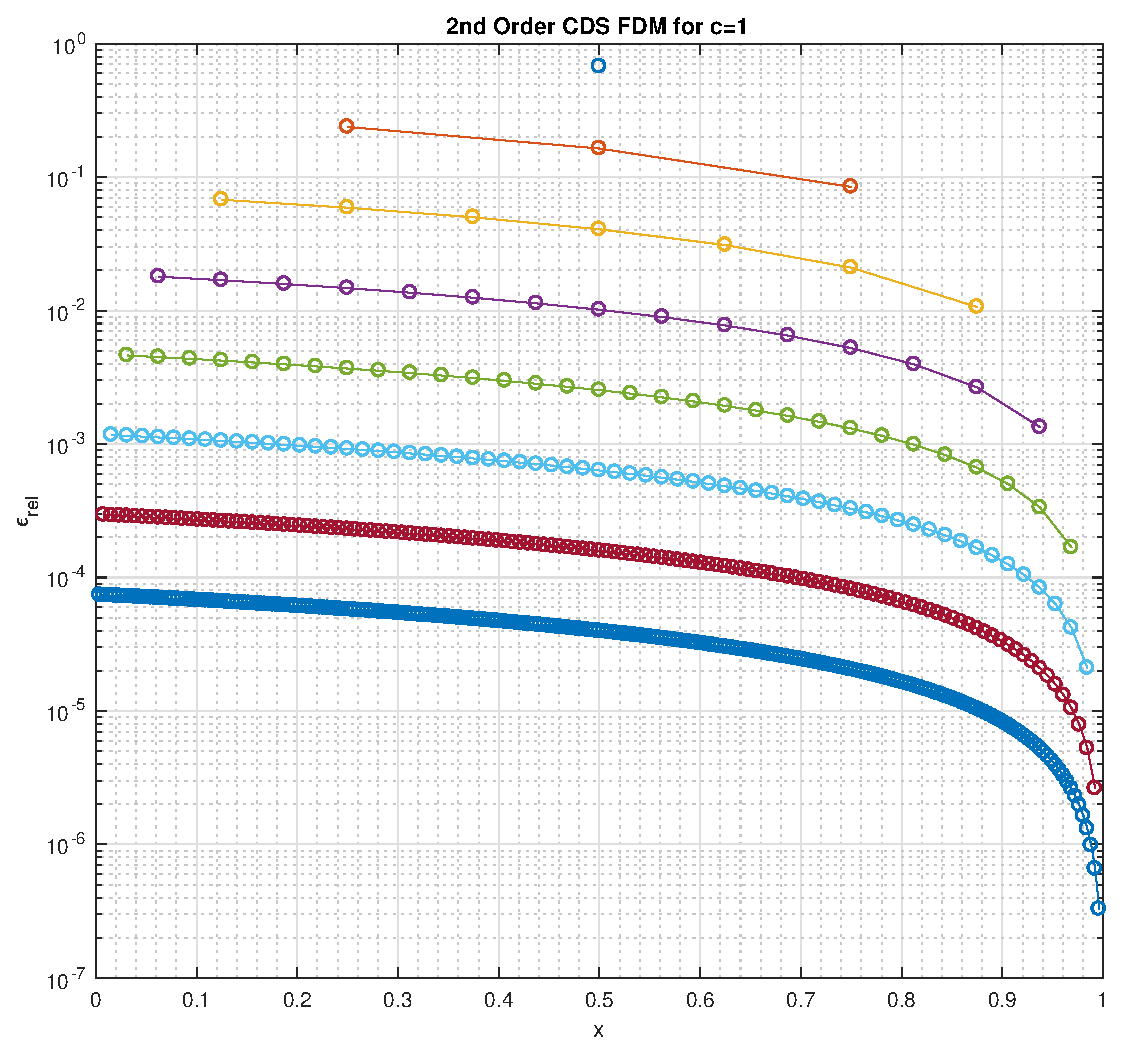
\includegraphics[width = 0.49\linewidth]{pointwise_error_2nd_order_cds_c_1}
		\caption{2nd-Order CDS FDM and Pointwise Error for $c = 1$}
	\end{center}
\end{figure}

\begin{figure}[H]
	\begin{center}
		\includegraphics[width = 0.49\linewidth]{solution_2nd_order_cds_c_2}
		\includegraphics[width = 0.49\linewidth]{pointwise_error_2nd_order_cds_c_2}
		\caption{2nd-Order CDS FDM and Pointwise Error for $c = 2$}
	\end{center}
\end{figure}

\begin{center}
	\includegraphics[height = 0.11\linewidth]{legend}
\end{center}

\newpage

\begin{figure}[H]
	\begin{center}
		\includegraphics[width = 0.49\linewidth]{solution_2nd_order_cds_c_5}
		\includegraphics[width = 0.49\linewidth]{pointwise_error_2nd_order_cds_c_5}
		\caption{2nd-Order CDS FDM and Pointwise Error for $c = 5$}
	\end{center}
\end{figure}

\begin{figure}[H]
	\begin{center}
		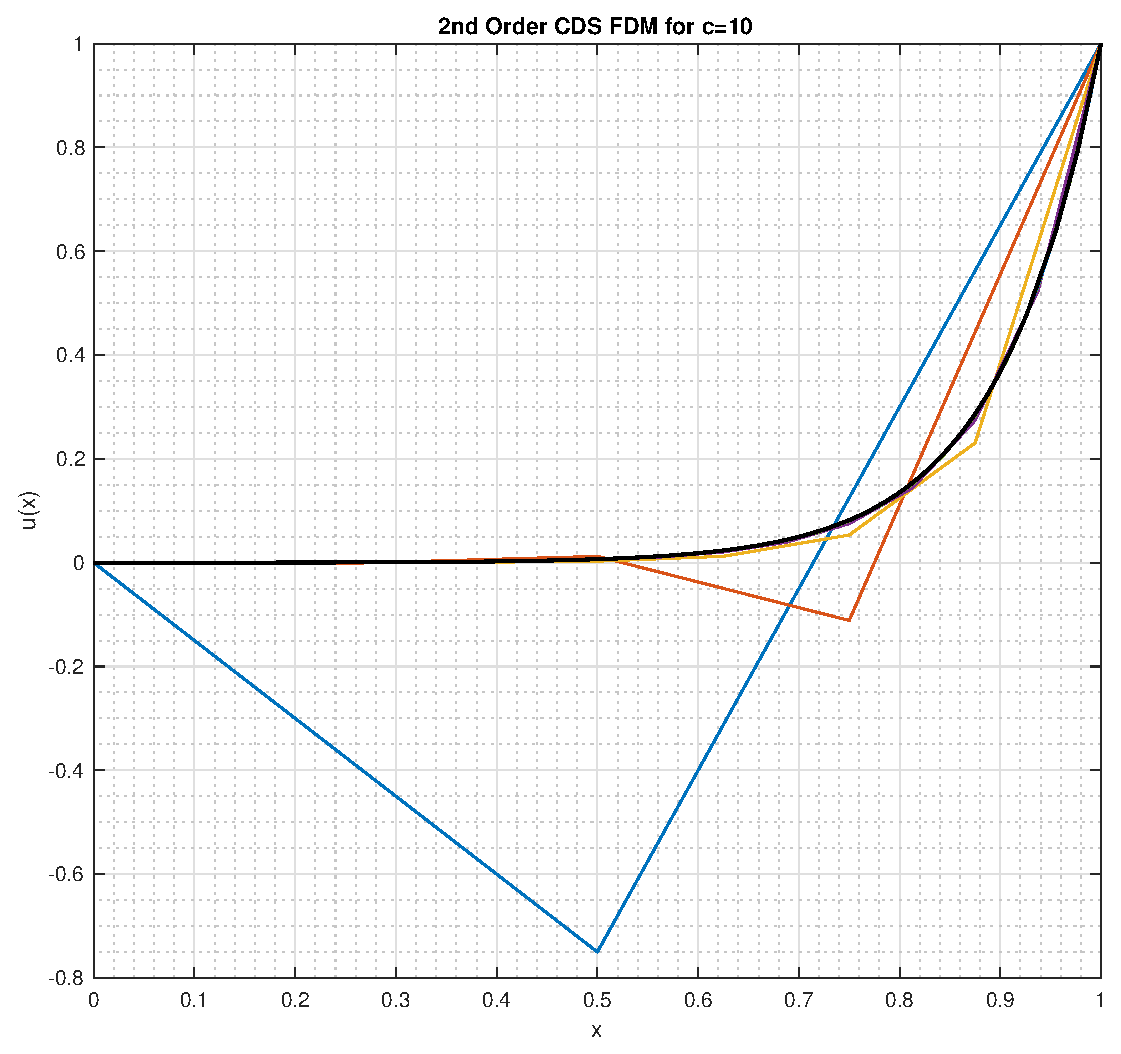
\includegraphics[width = 0.49\linewidth]{solution_2nd_order_cds_c_10}
		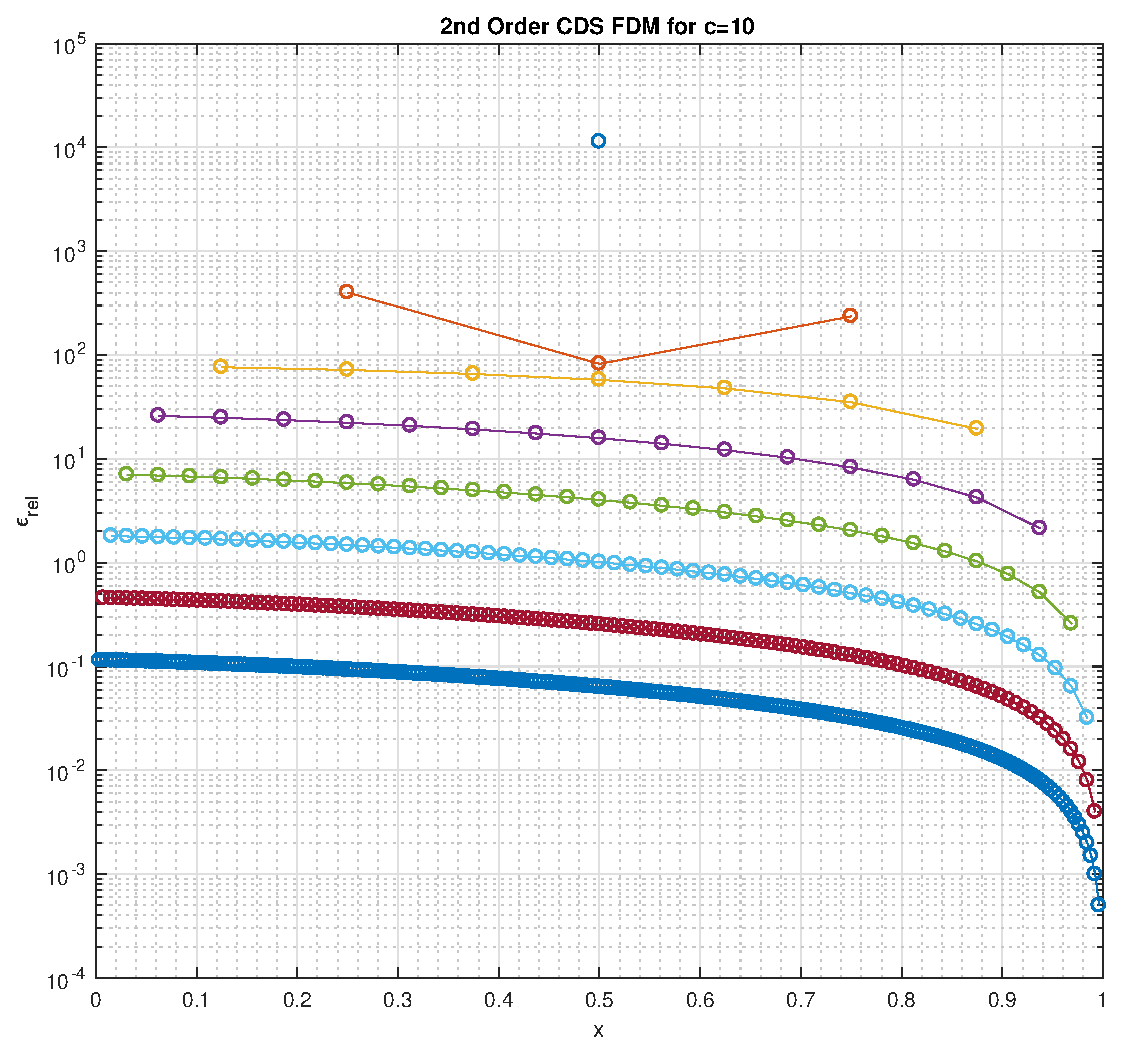
\includegraphics[width = 0.49\linewidth]{pointwise_error_2nd_order_cds_c_10}
		\caption{2nd-Order CDS FDM and Pointwise Error for $c = 10$}
	\end{center}
\end{figure}

\begin{center}
	\includegraphics[height = 0.25\linewidth]{legend}
\end{center}

\newpage

\begin{figure}[H]
	\begin{center}
		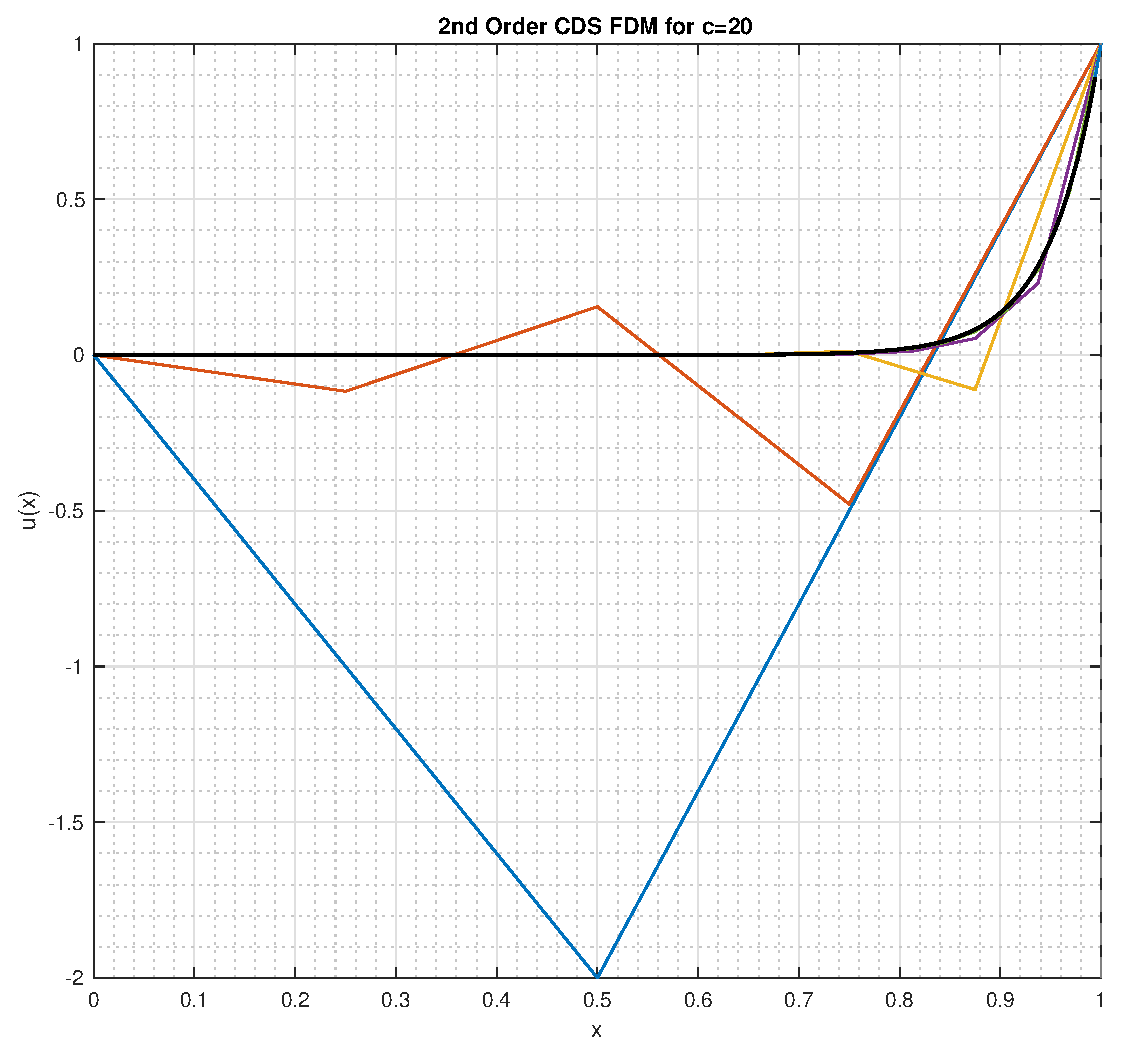
\includegraphics[width = 0.49\linewidth]{solution_2nd_order_cds_c_20}
		\includegraphics[width = 0.49\linewidth]{pointwise_error_2nd_order_cds_c_20}
		\caption{2nd-Order CDS FDM and Pointwise Error for $c = 20$}
	\end{center}
\end{figure}

\begin{figure}[H]
	\begin{center}
		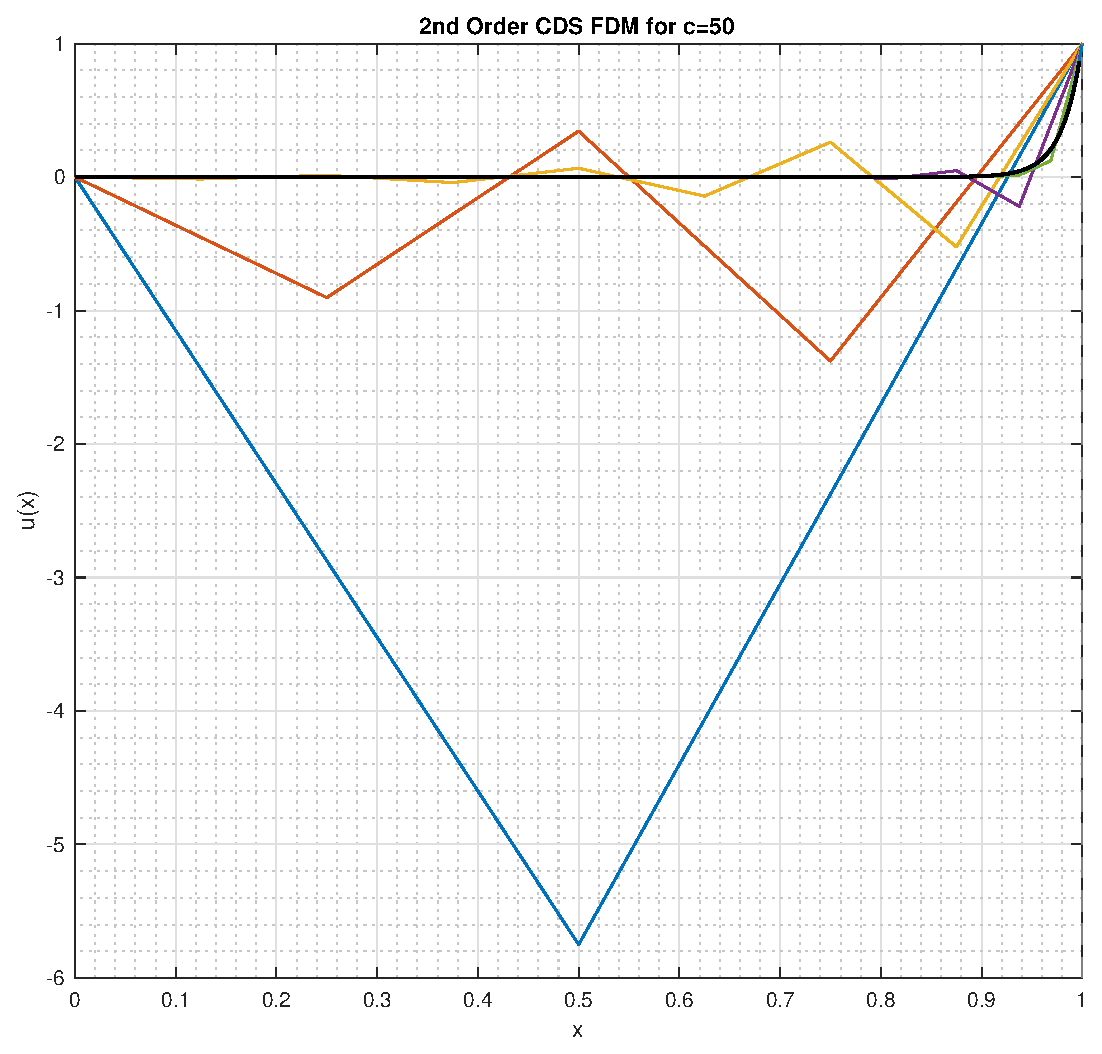
\includegraphics[width = 0.49\linewidth]{solution_2nd_order_cds_c_50}
		\includegraphics[width = 0.49\linewidth]{pointwise_error_2nd_order_cds_c_50}
		\caption{2nd-Order CDS FDM and Pointwise Error for $c = 50$}
	\end{center}
\end{figure}

\begin{center}
	\includegraphics[height = 0.25\linewidth]{legend}
\end{center}

\newpage

\subsubsection{4th-Order Central Difference Scheme Finite Difference Method}

\begin{figure}[H]
	\begin{center}
		\includegraphics[width = 0.49\linewidth]{solution_4th_order_cds_c_1}
		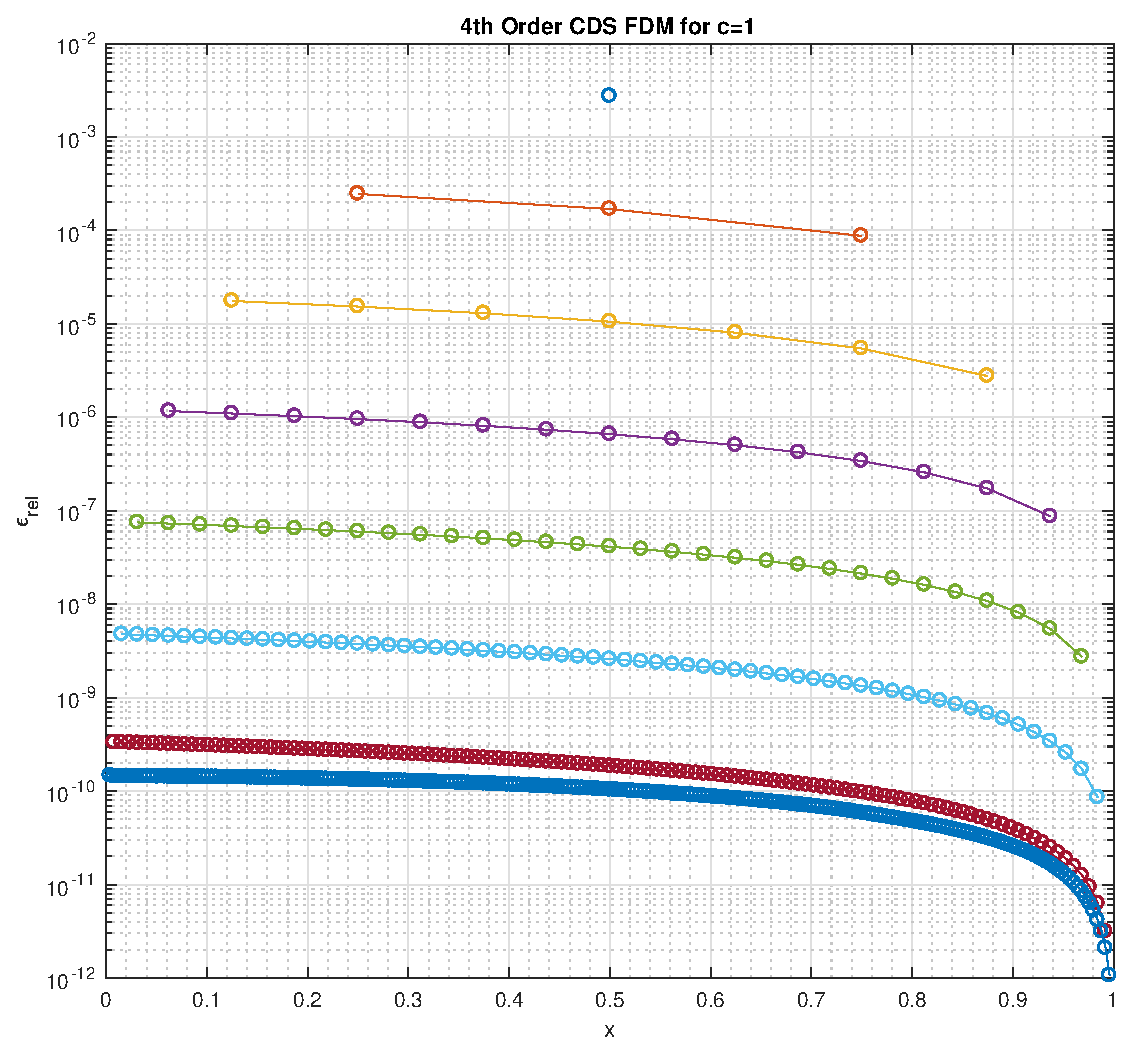
\includegraphics[width = 0.49\linewidth]{pointwise_error_4th_order_cds_c_1}
		\caption{4th-Order CDS FDM and Pointwise Error for $c = 1$}
	\end{center}
\end{figure}

\begin{figure}[H]
	\begin{center}
		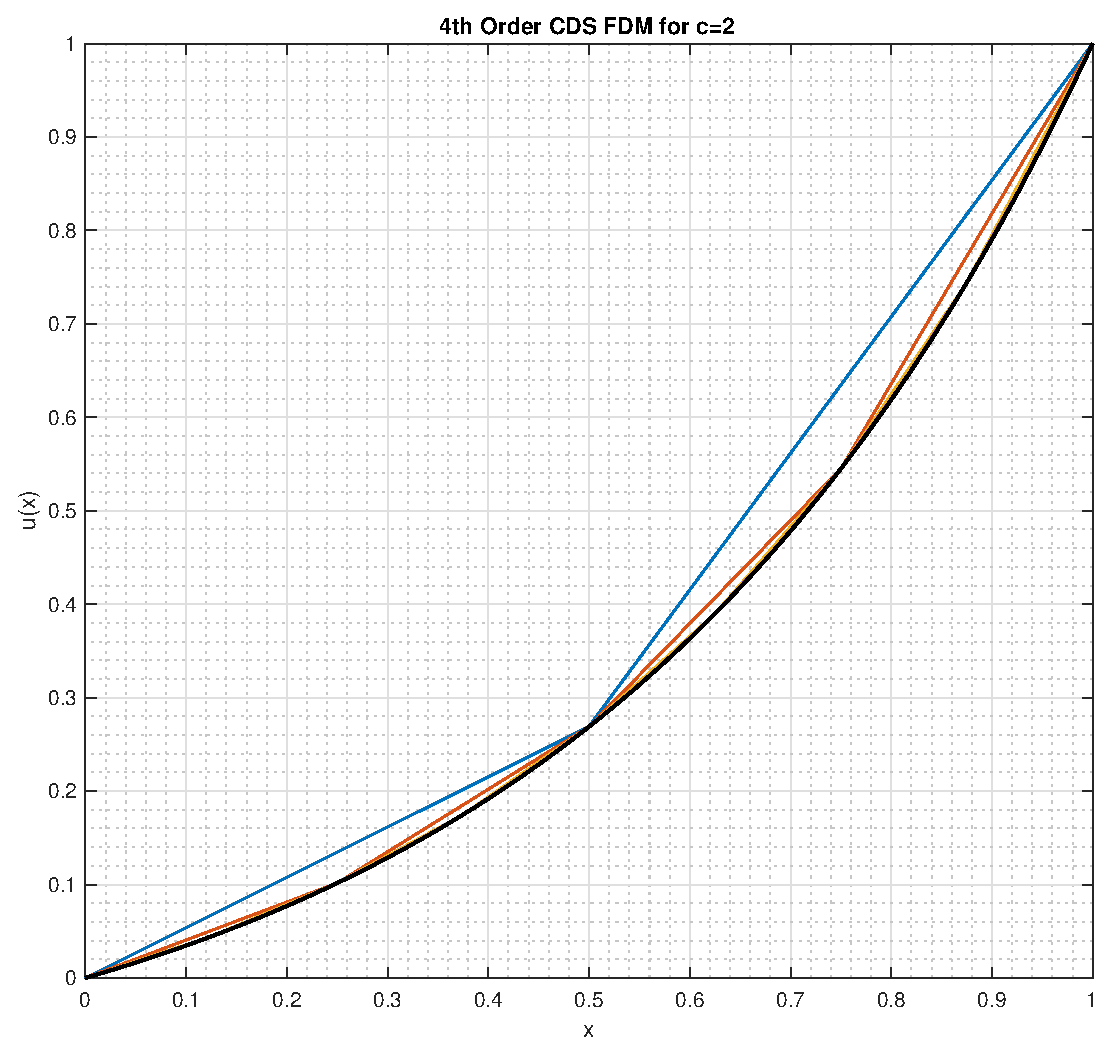
\includegraphics[width = 0.49\linewidth]{solution_4th_order_cds_c_2}
		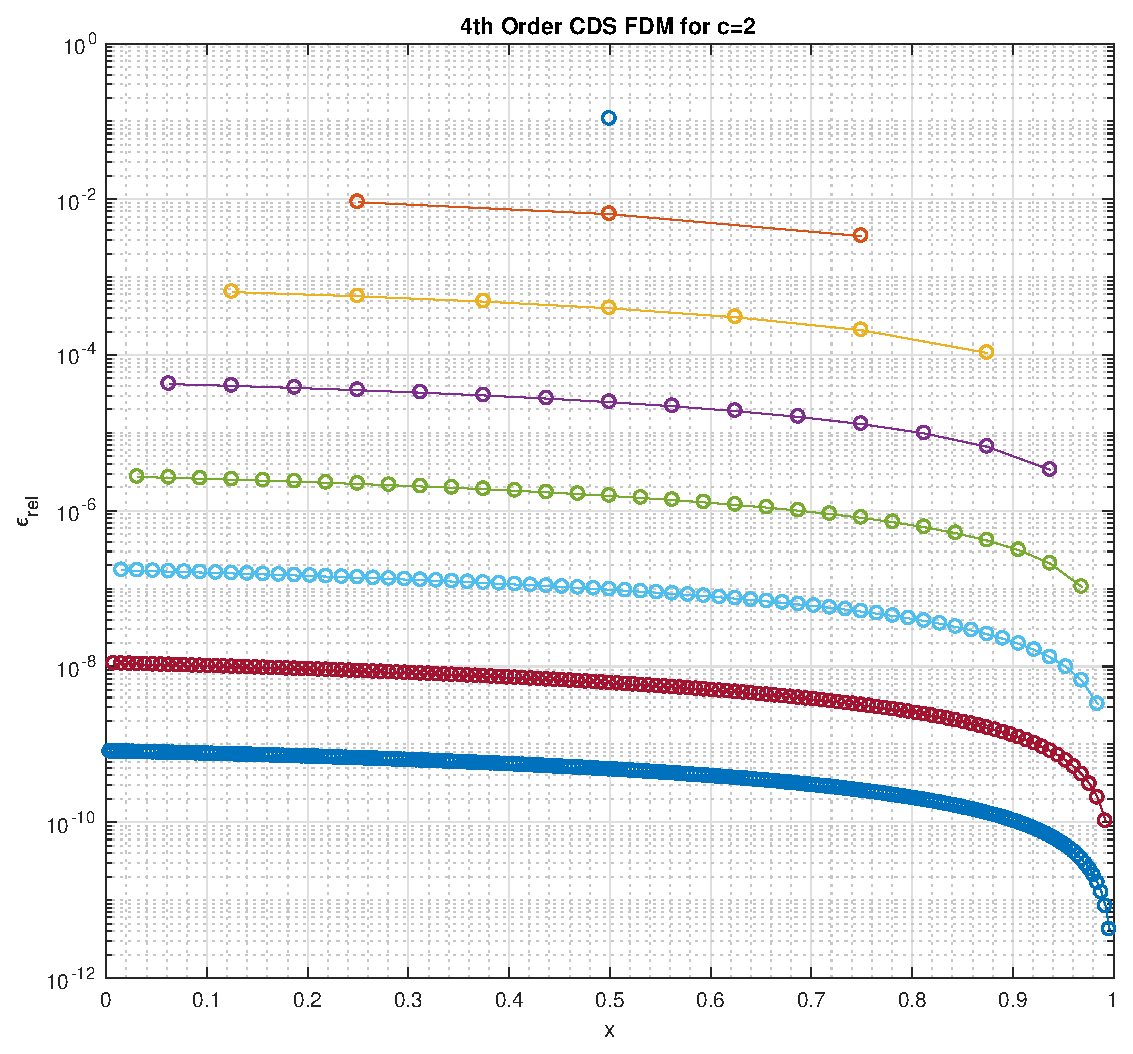
\includegraphics[width = 0.49\linewidth]{pointwise_error_4th_order_cds_c_2}
		\caption{4th-Order CDS FDM and Pointwise Error for $c = 2$}
	\end{center}
\end{figure}

\begin{center}
	\includegraphics[height = 0.17\linewidth]{legend}
\end{center}

\newpage

\begin{figure}[H]
	\begin{center}
		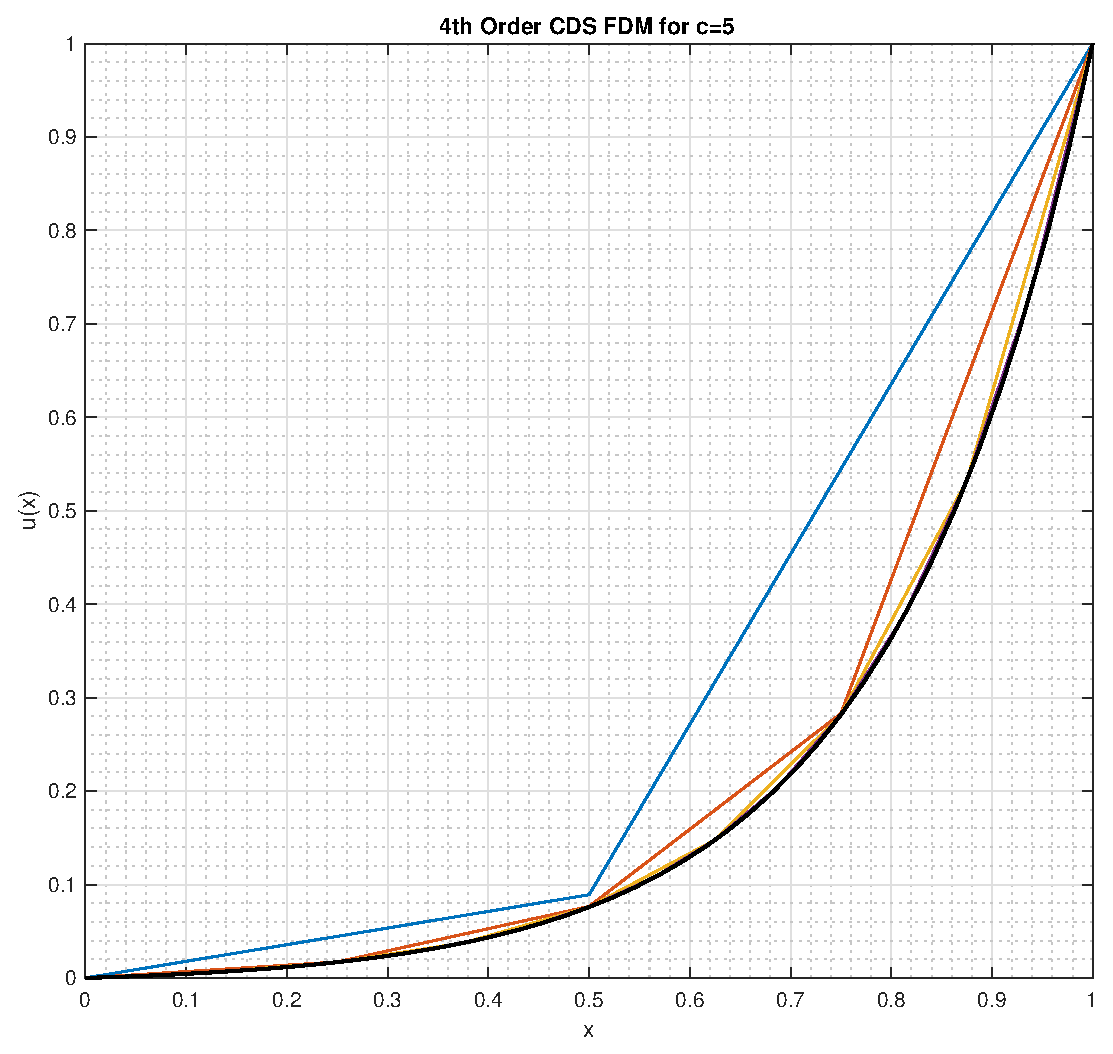
\includegraphics[width = 0.49\linewidth]{solution_4th_order_cds_c_5}
		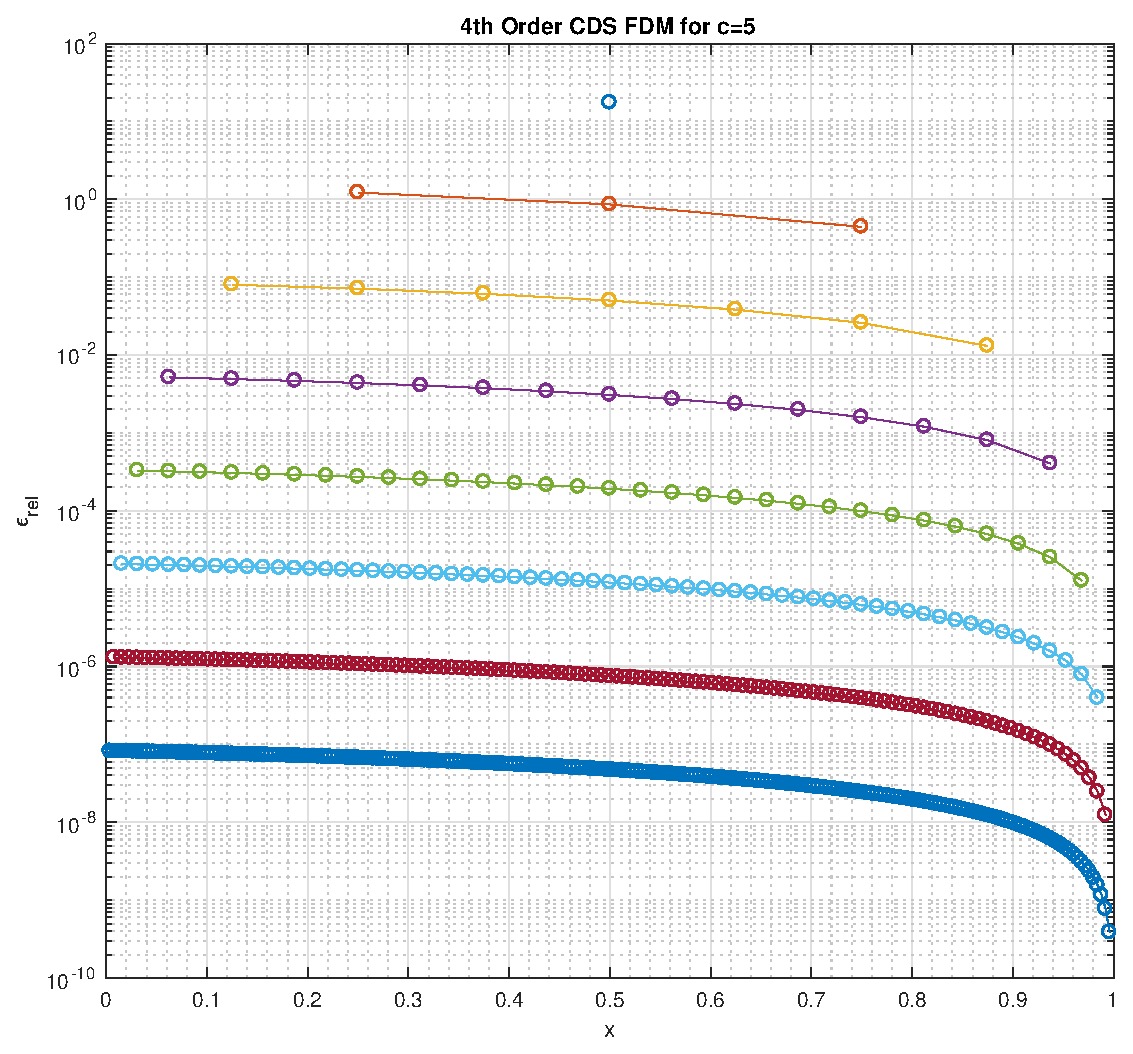
\includegraphics[width = 0.49\linewidth]{pointwise_error_4th_order_cds_c_5}
		\caption{4th-Order CDS FDM and Pointwise Error for $c = 5$}
	\end{center}
\end{figure}

\begin{figure}[H]
	\begin{center}
		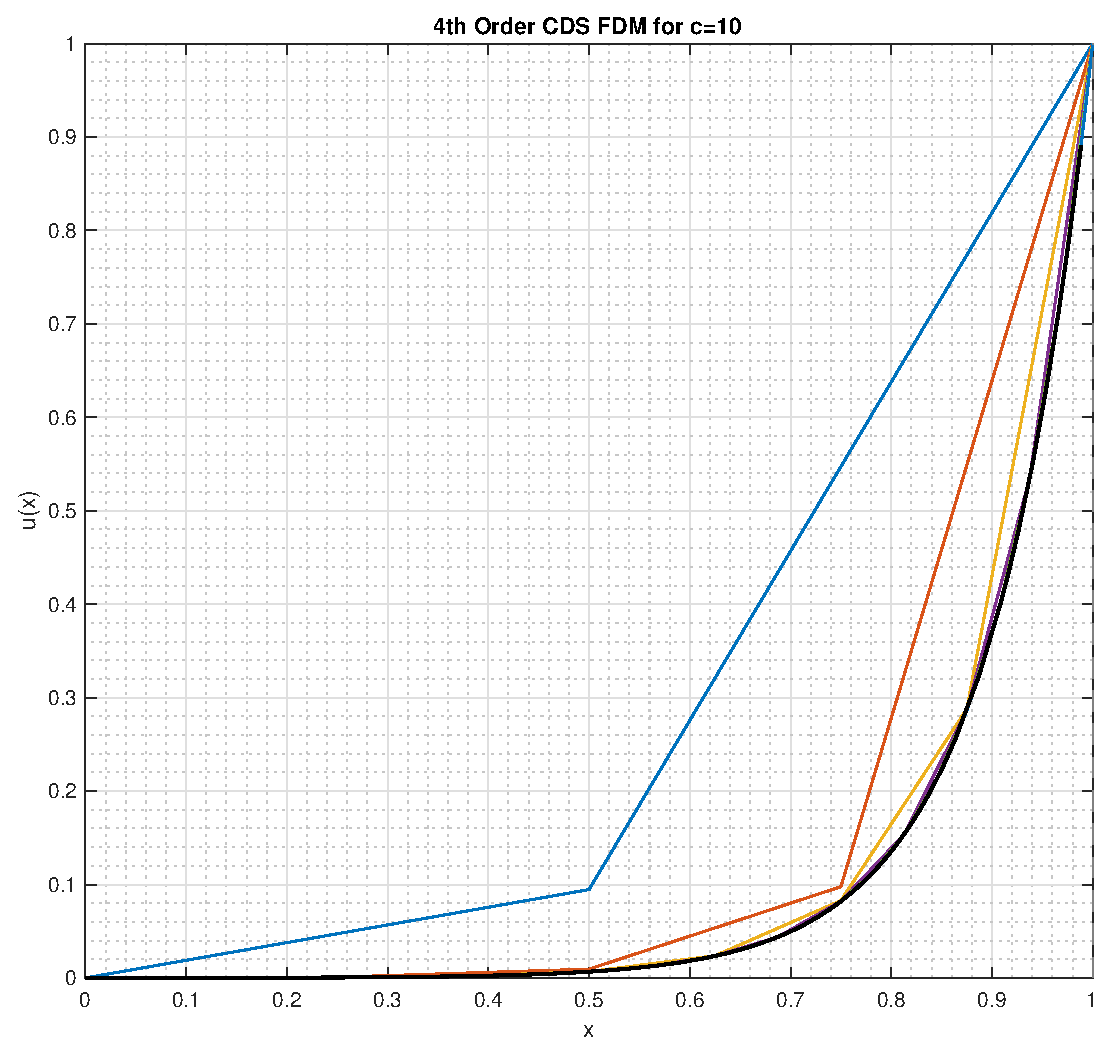
\includegraphics[width = 0.49\linewidth]{solution_4th_order_cds_c_10}
		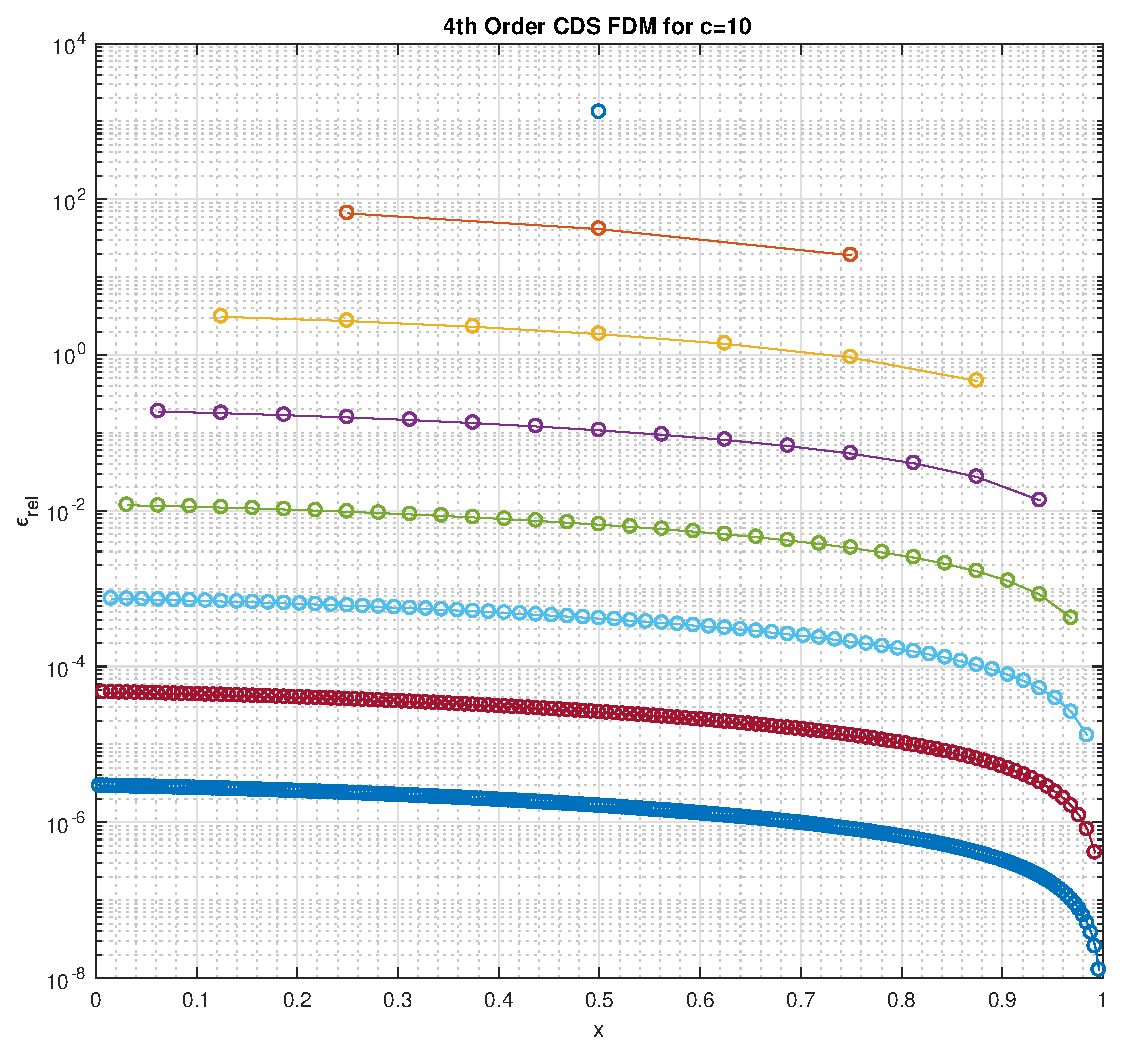
\includegraphics[width = 0.49\linewidth]{pointwise_error_4th_order_cds_c_10}
		\caption{4th-Order CDS FDM and Pointwise Error for $c = 10$}
	\end{center}
\end{figure}

\begin{center}
	\includegraphics[height = 0.25\linewidth]{legend}
\end{center}

\newpage

\begin{figure}[H]
	\begin{center}
		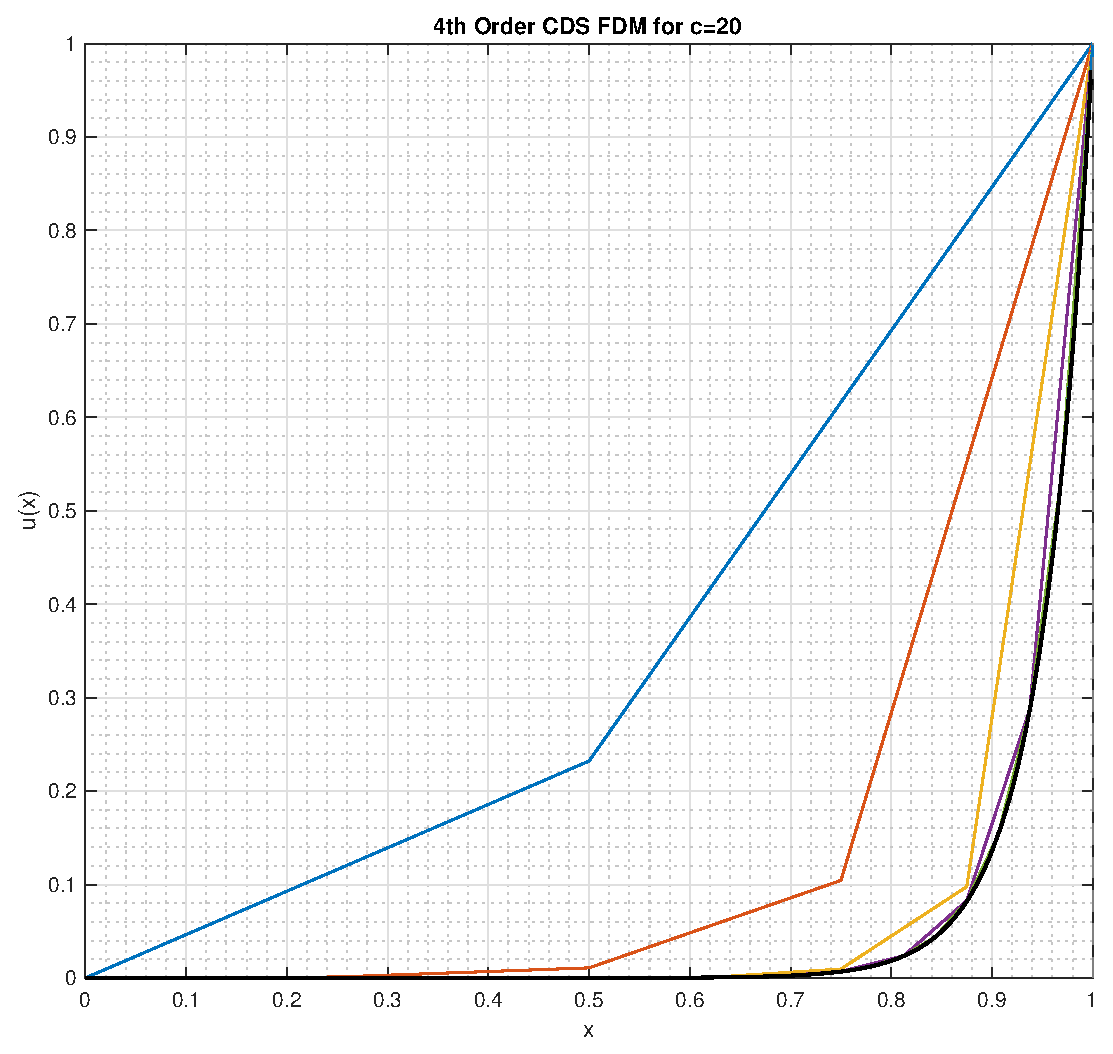
\includegraphics[width = 0.49\linewidth]{solution_4th_order_cds_c_20}
		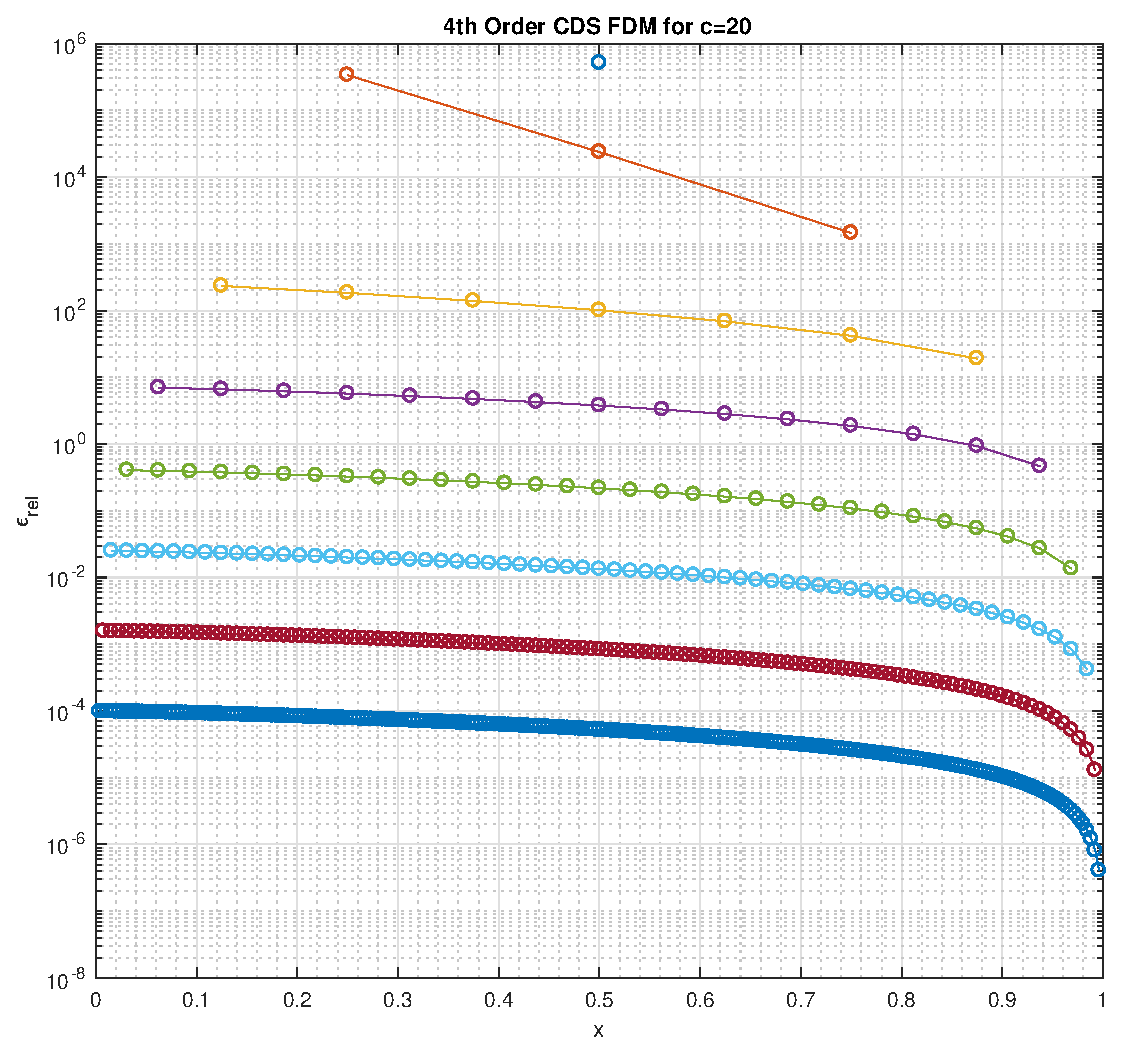
\includegraphics[width = 0.49\linewidth]{pointwise_error_4th_order_cds_c_20}
		\caption{4th-Order CDS FDM and Pointwise Error for $c = 20$}
	\end{center}
\end{figure}

\begin{figure}[H]
	\begin{center}
		\includegraphics[width = 0.49\linewidth]{solution_4th_order_cds_c_50}
		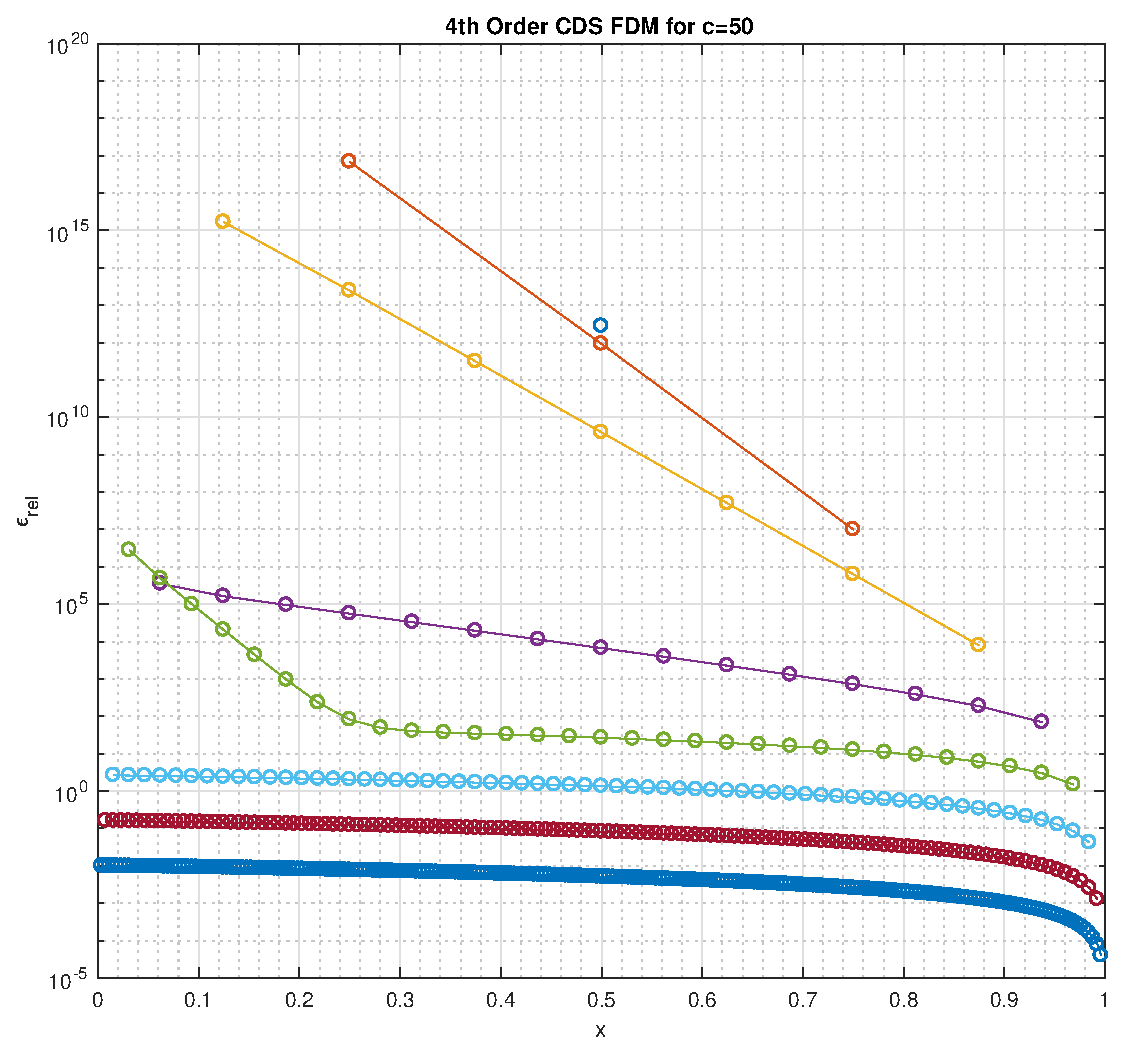
\includegraphics[width = 0.49\linewidth]{pointwise_error_4th_order_cds_c_50}
		\caption{4th-Order CDS FDM and Pointwise Error for $c = 50$}
	\end{center}
\end{figure}

\begin{center}
	\includegraphics[height = 0.25\linewidth]{legend}
\end{center}

\subsubsection{1st-Order Upwind Scheme Finite Difference Method}

\begin{figure}[H]
	\begin{center}
		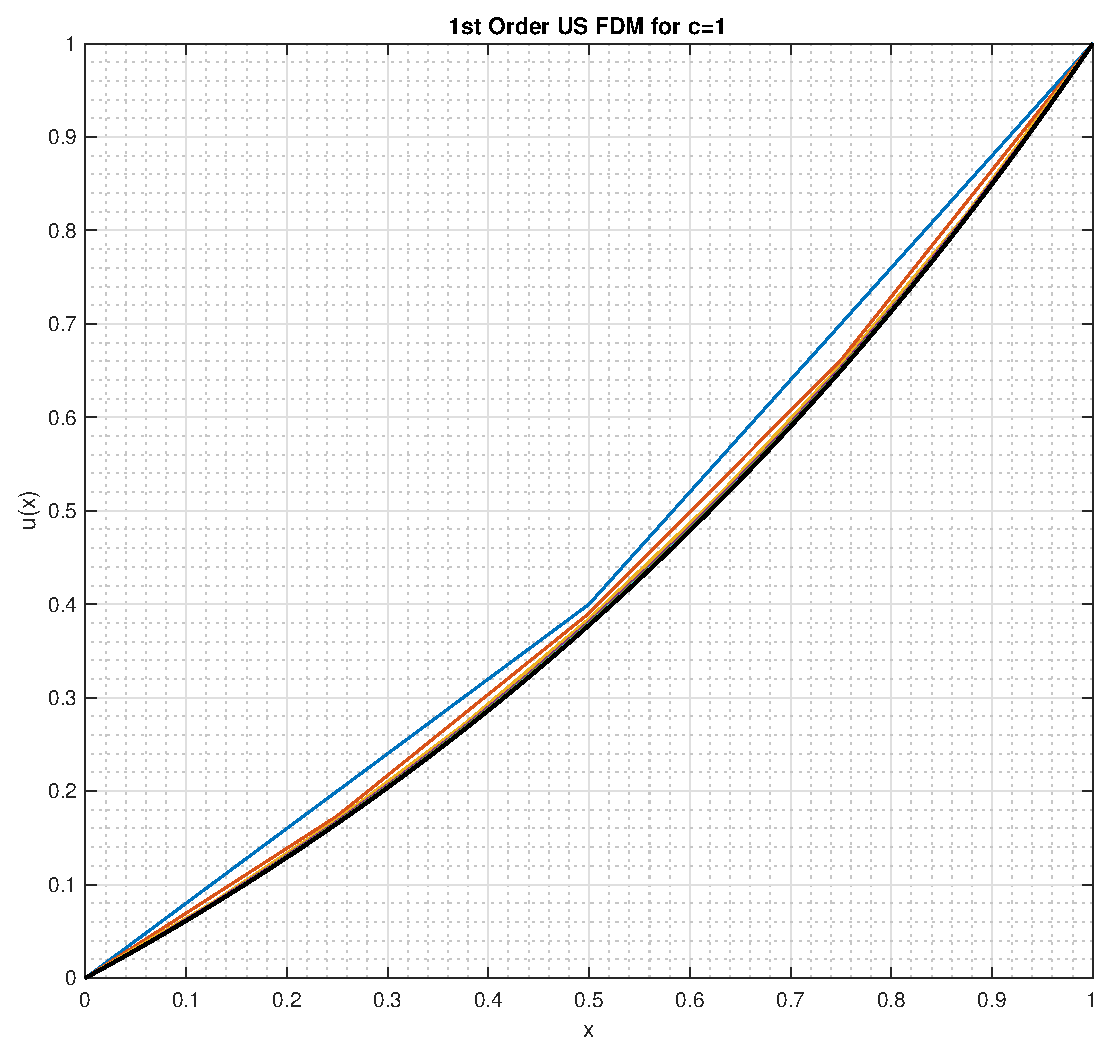
\includegraphics[width = 0.49\linewidth]{solution_1st_order_us_c_1}
		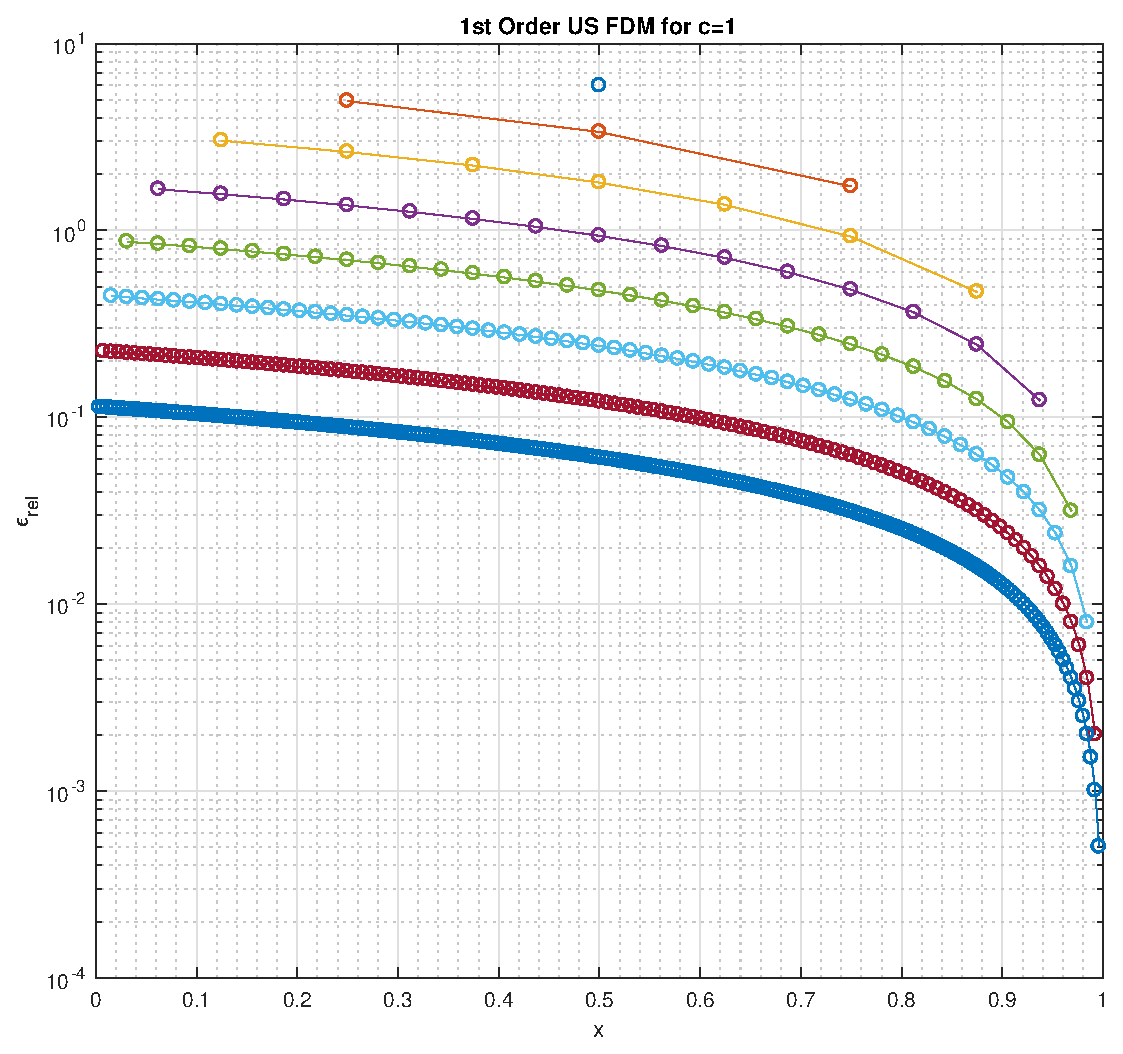
\includegraphics[width = 0.49\linewidth]{pointwise_error_1st_order_us_c_1}
		\caption{1st-Order US FDM and Pointwise Error for $c = 1$}
	\end{center}
\end{figure}

\begin{figure}[H]
	\begin{center}
		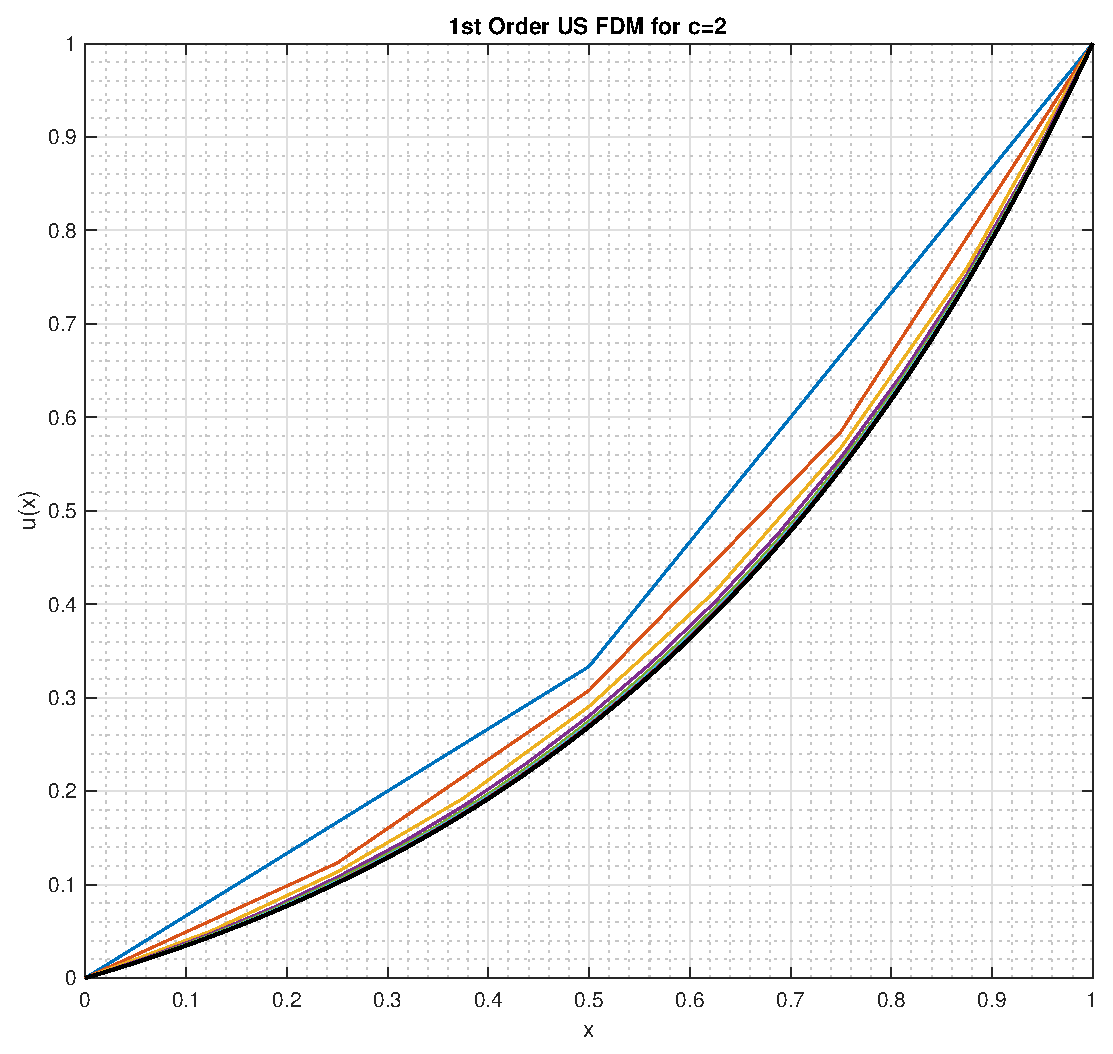
\includegraphics[width = 0.49\linewidth]{solution_1st_order_us_c_2}
		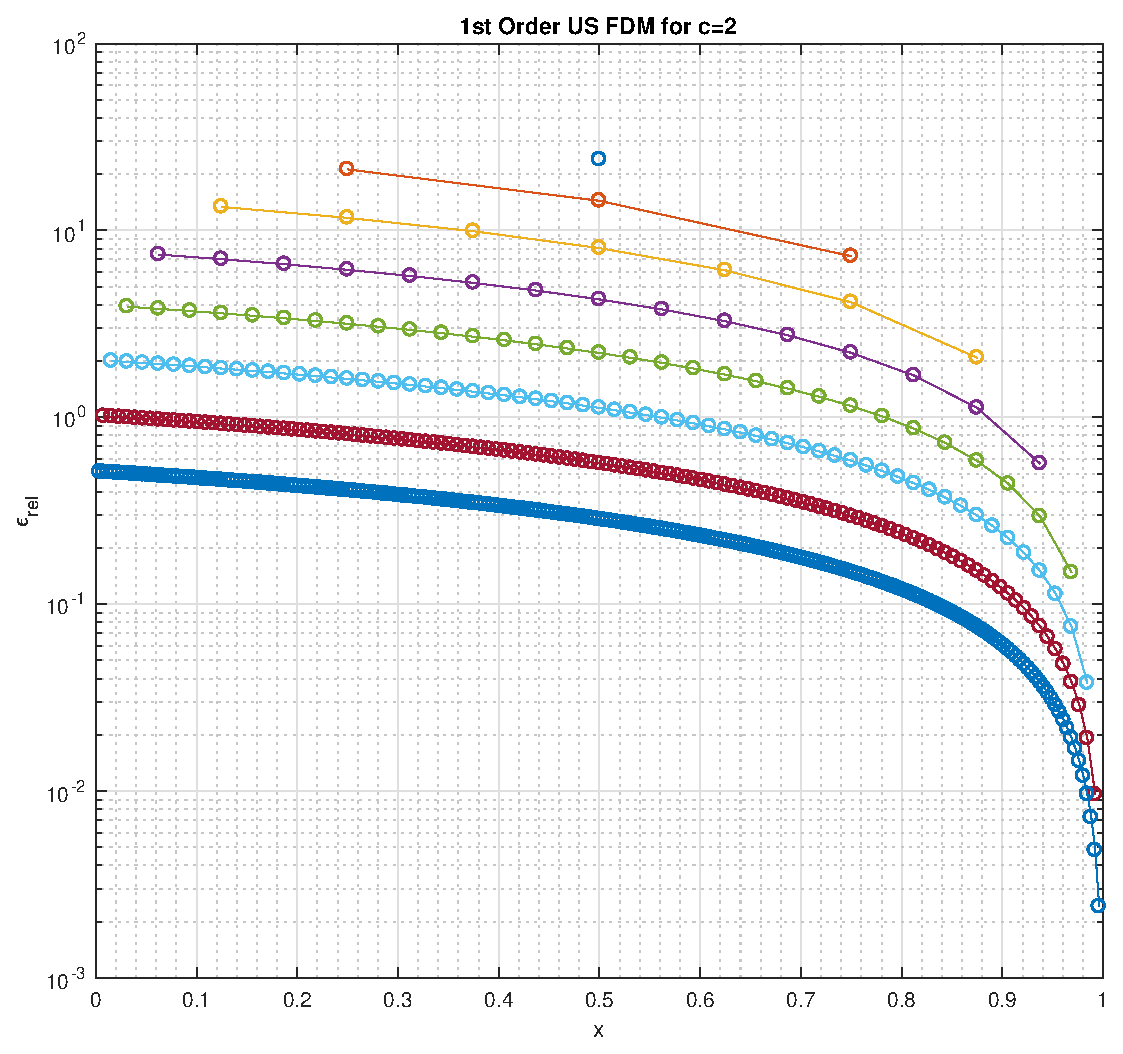
\includegraphics[width = 0.49\linewidth]{pointwise_error_1st_order_us_c_2}
		\caption{1st-Order US FDM and Pointwise Error for $c = 2$}
	\end{center}
\end{figure}

\begin{center}
	\includegraphics[height = 0.17\linewidth]{legend}
\end{center}

\newpage

\begin{figure}[H]
	\begin{center}
		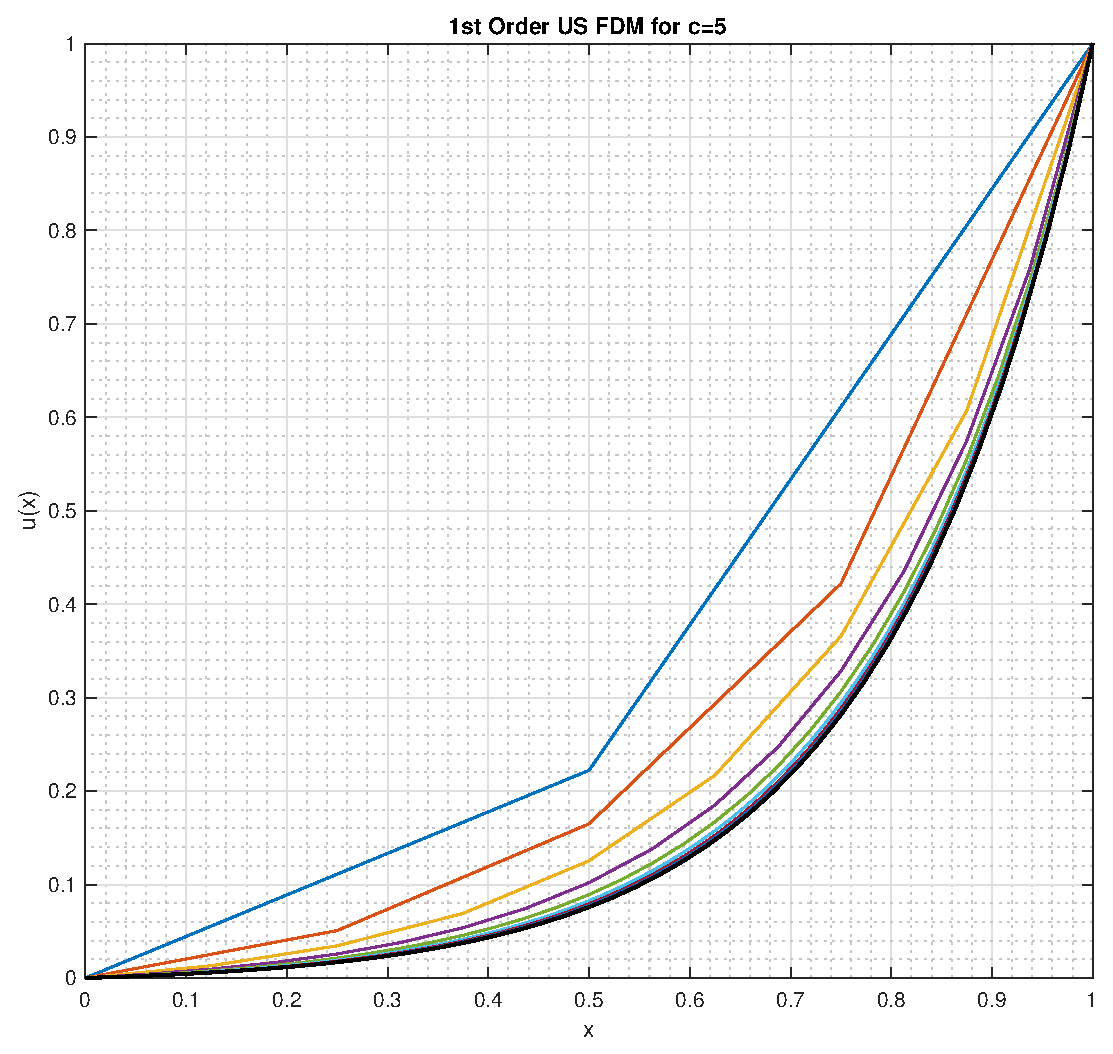
\includegraphics[width = 0.49\linewidth]{solution_1st_order_us_c_5}
		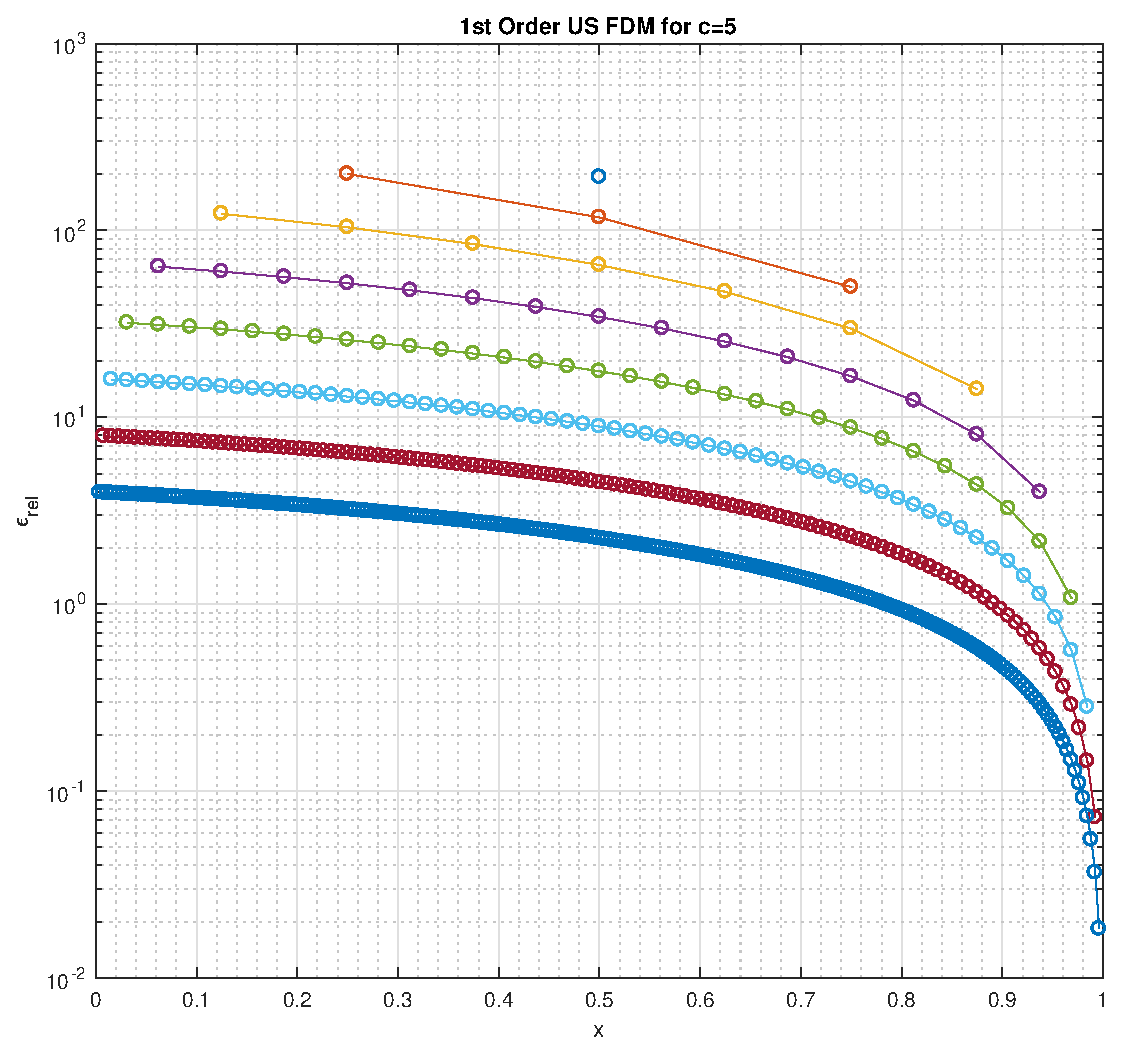
\includegraphics[width = 0.49\linewidth]{pointwise_error_1st_order_us_c_5}
		\caption{1st-Order US FDM and Pointwise Error for $c = 5$}
	\end{center}
\end{figure}

\begin{figure}[H]
	\begin{center}
		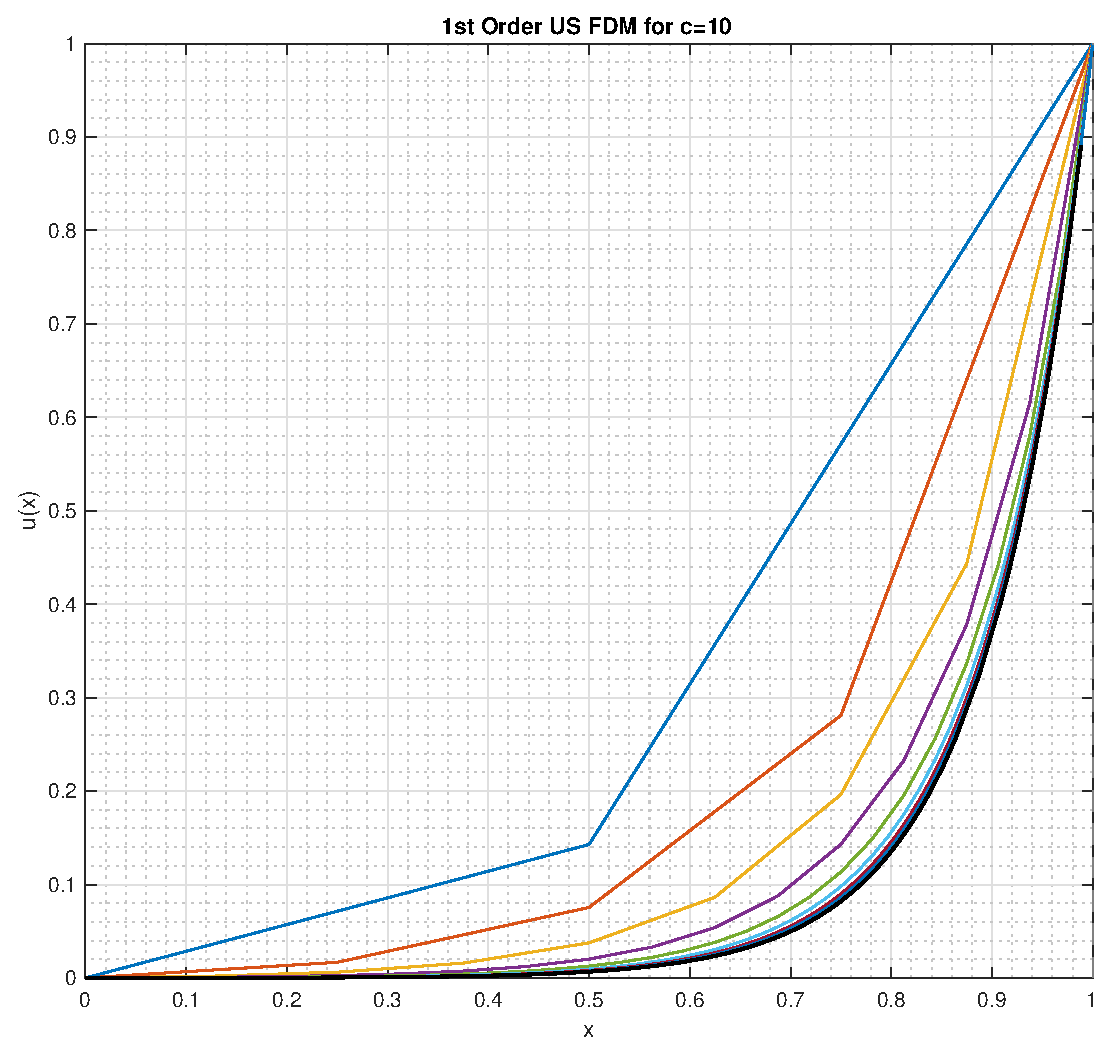
\includegraphics[width = 0.49\linewidth]{solution_1st_order_us_c_10}
		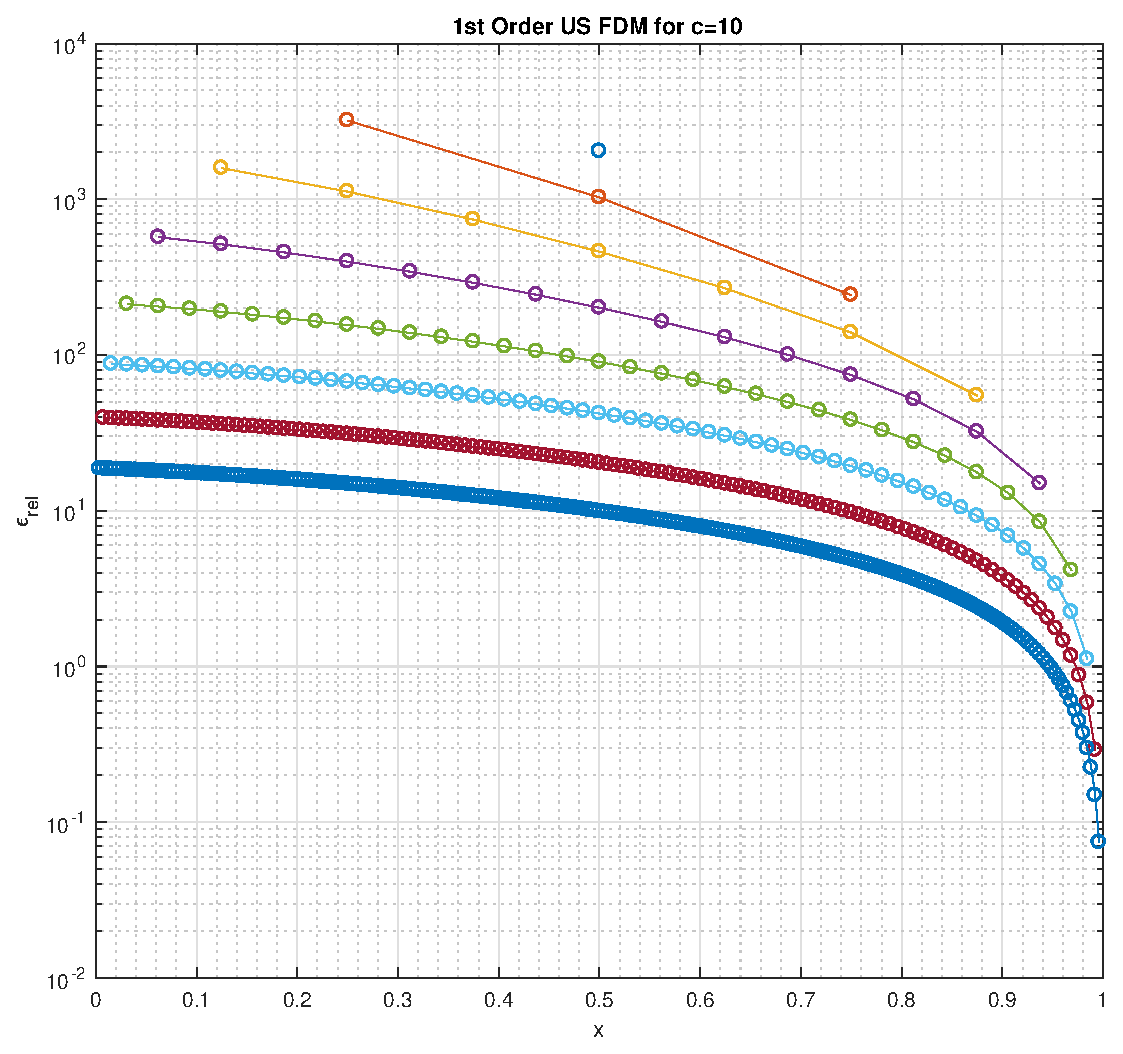
\includegraphics[width = 0.49\linewidth]{pointwise_error_1st_order_us_c_10}
		\caption{1st-Order US FDM and Pointwise Error for $c = 10$}
	\end{center}
\end{figure}

\begin{center}
	\includegraphics[height = 0.25\linewidth]{legend}
\end{center}

\newpage

\begin{figure}[H]
	\begin{center}
		\includegraphics[width = 0.49\linewidth]{solution_1st_order_us_c_20}
		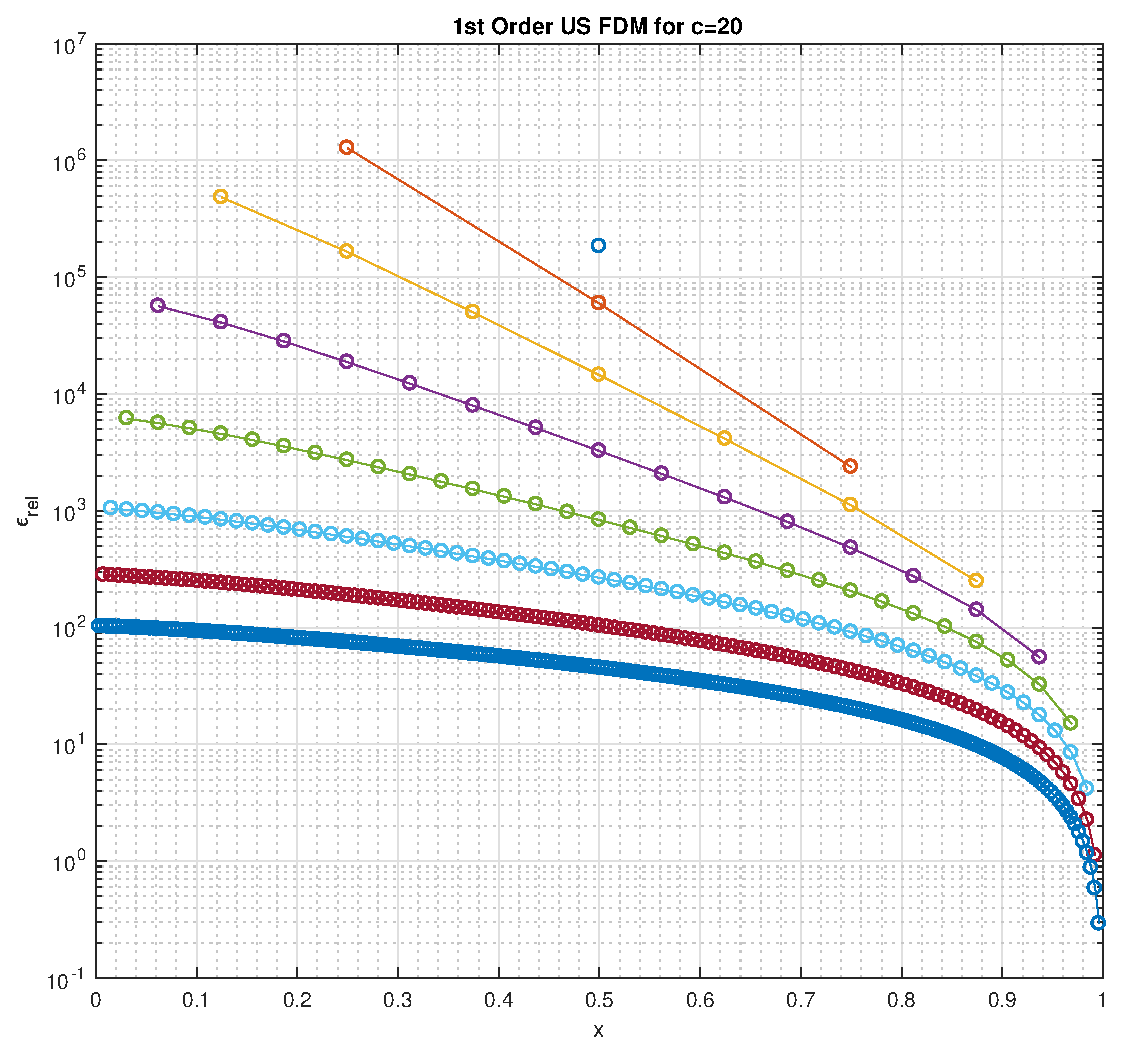
\includegraphics[width = 0.49\linewidth]{pointwise_error_1st_order_us_c_20}
		\caption{1st-Order US FDM and Pointwise Error for $c = 20$}
	\end{center}
\end{figure}

\begin{figure}[H]
	\begin{center}
		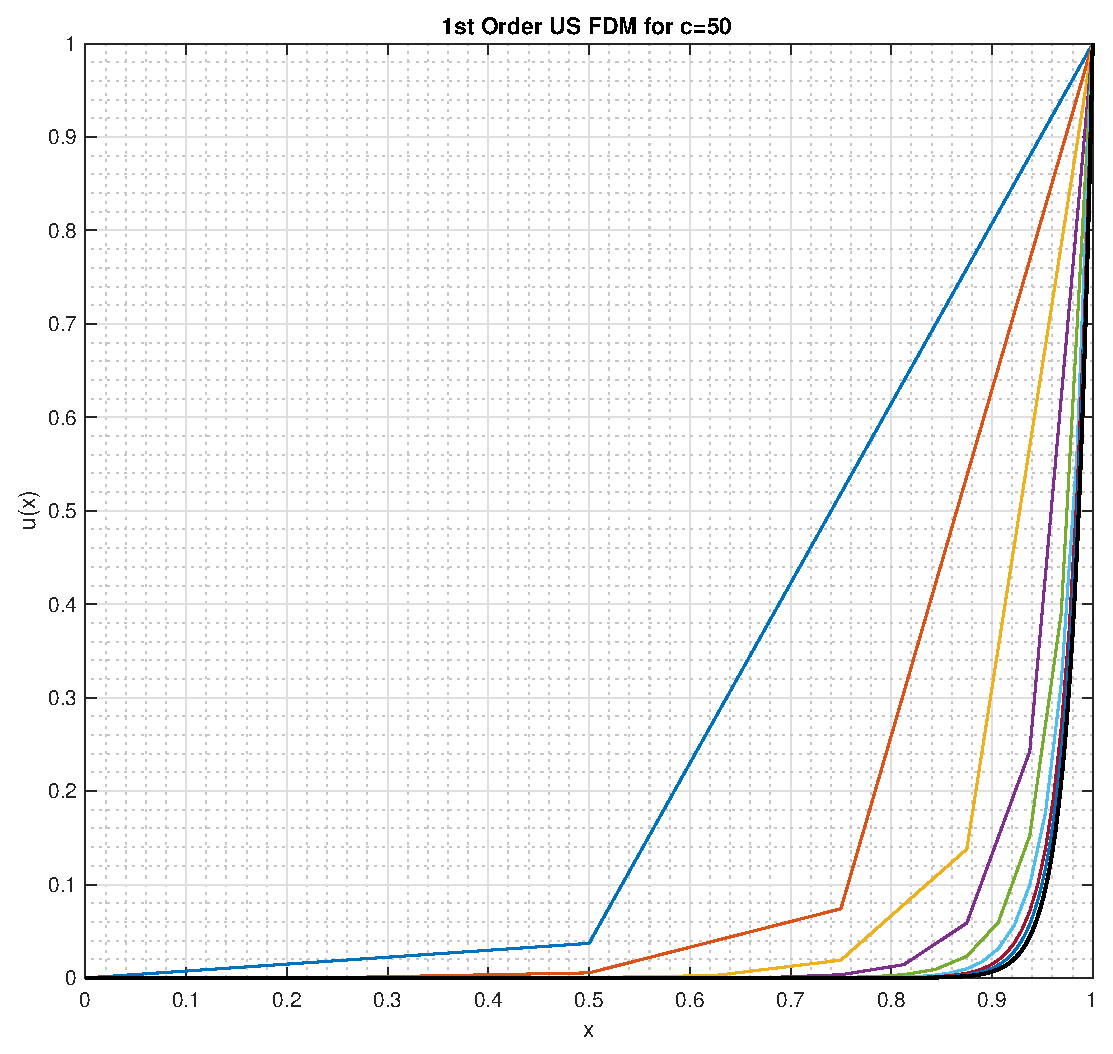
\includegraphics[width = 0.49\linewidth]{solution_1st_order_us_c_50}
		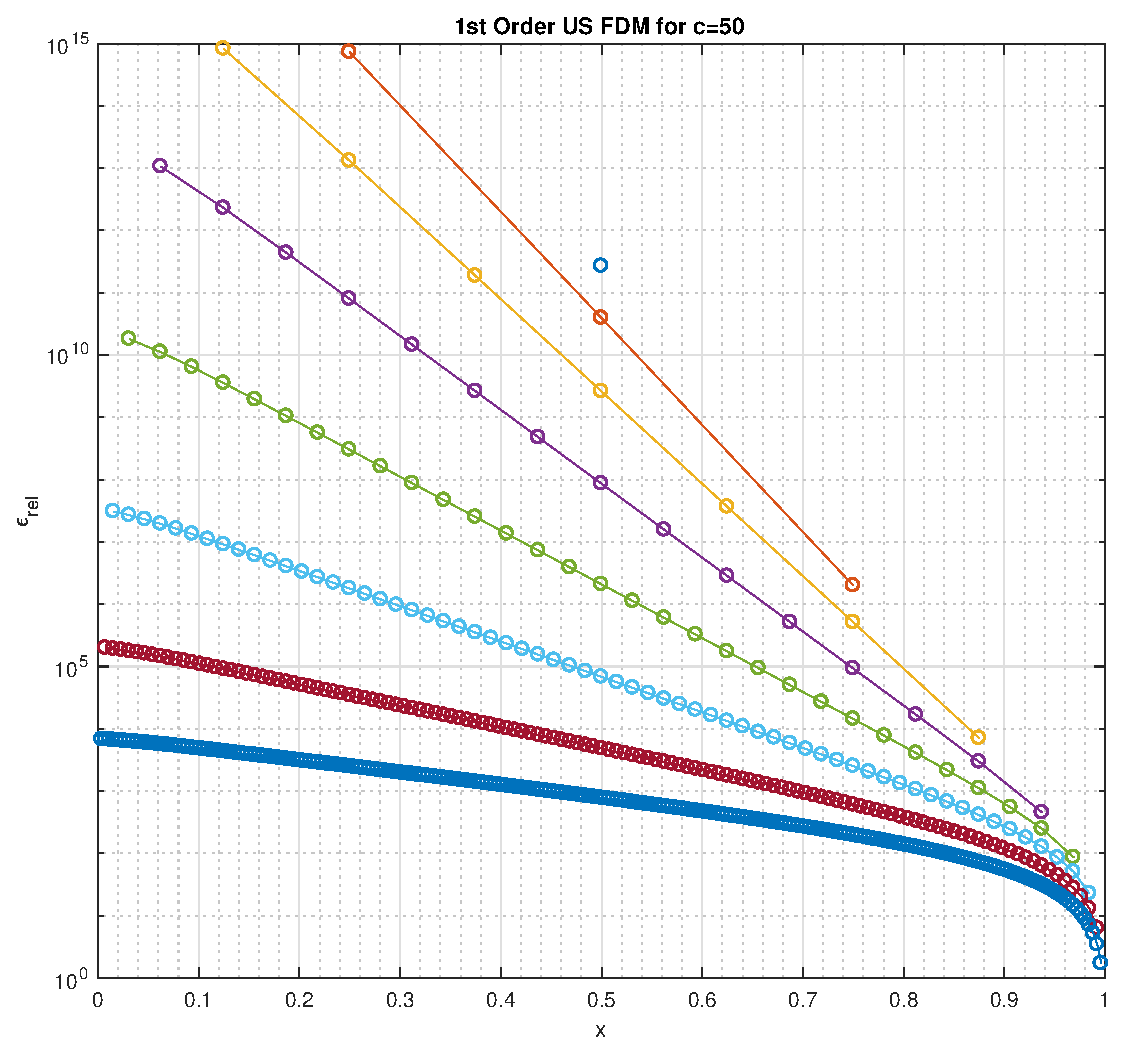
\includegraphics[width = 0.49\linewidth]{pointwise_error_1st_order_us_c_50}
		\caption{1st-Order US FDM and Pointwise Error for $c = 50$}
	\end{center}
\end{figure}

\begin{center}
	\includegraphics[height = 0.25\linewidth]{legend}
\end{center}

\newpage

\subsection{Quantity of Interest Results}

\subsubsection{2nd-Order Central Difference Scheme Finite Difference Method}

\begin{table}[H]
	\caption{Quantity of Interest Values for 2nd-Order CDS FDM - I}	
	\input{qoi_1_table_2nd_order_cds.tex}
\end{table}

\newpage

\begin{table}[H]
	\caption{Quantity of Interest Values for 2nd-Order CDS FDM - II}	
	\input{qoi_2_table_2nd_order_cds.tex}
\end{table}

\newpage

\subsubsection{4th-Order Central Difference Scheme Finite Difference Method}

\begin{table}[H]
	\caption{Quantity of Interest Values for 4th-Order CDS FDM - I}
	\begin{tabular}{|c|c|c|c|c|c|c|c|c|c|}
\hline
\textbf{$\Delta x$}&\textbf{$u'_{c=1}(1)$}&\textbf{$u'_{c=2}(1)$}&\textbf{$u'_{c=5}(1)$}&\textbf{$\bar{u}'_{c=1}(1)$}&\textbf{$\bar{u}'_{c=2}(1)$}&\textbf{$\bar{u}'_{c=5}(1)$}&\textbf{$\epsilon'_{rel,c=1}$}&\textbf{$\epsilon'_{rel,c=2}$}&\textbf{$\epsilon'_{rel,c=5}$}\\\hline
0.5000&1.5829&2.3385&12.9559&1.5820&2.3130&5.0339&0.0594&1.0993&157.3713\\\hline
0.2500&1.5820&2.3144&5.1772&1.5820&2.3130&5.0339&0.0034&0.0570&2.8461\\\hline
0.1250&1.5820&2.3131&5.0410&1.5820&2.3130&5.0339&0.0002&0.0032&0.1400\\\hline
0.0625&1.5820&2.3130&5.0343&1.5820&2.3130&5.0339&0.0000&0.0002&0.0077\\\hline
0.0312&1.5820&2.3130&5.0339&1.5820&2.3130&5.0339&0.0000&0.0000&0.0004\\\hline
0.0156&1.5820&2.3130&5.0339&1.5820&2.3130&5.0339&0.0000&0.0000&0.0000\\\hline
0.0078&1.5820&2.3130&5.0339&1.5820&2.3130&5.0339&0.0000&0.0000&0.0000\\\hline
0.0039&1.5820&2.3130&5.0339&1.5820&2.3130&5.0339&0.0000&0.0000&0.0000\\\hline
0.0020&1.5820&2.3130&5.0339&1.5820&2.3130&5.0339&0.0000&0.0000&0.0000\\\hline
0.0010&1.5820&2.3130&5.0339&1.5820&2.3130&5.0339&0.0000&0.0000&0.0000\\\hline
0.0005&1.5820&2.3130&5.0339&1.5820&2.3130&5.0339&0.0000&0.0000&0.0000\\\hline
0.0002&1.5820&2.3130&5.0339&1.5820&2.3130&5.0339&0.0000&0.0000&0.0000\\\hline
0.0001&1.5820&2.3130&5.0339&1.5820&2.3130&5.0339&0.0000&0.0000&0.0000\\\hline
0.0001&1.5820&2.3130&5.0339&1.5820&2.3130&5.0339&0.0000&0.0000&0.0000\\\hline
0.0000&1.5820&2.3130&5.0339&1.5820&2.3130&5.0339&0.0000&0.0000&0.0000\\\hline
0.0000&1.5820&2.3130&5.0339&1.5820&2.3130&5.0339&0.0000&0.0000&0.0000\\\hline
0.0000&1.5820&2.3130&5.0339&1.5820&2.3130&5.0339&0.0000&0.0000&0.0000\\\hline
0.0000&1.5820&2.3130&5.0339&1.5820&2.3130&5.0339&0.0002&0.0001&0.0000\\\hline
0.0000&1.5820&2.3130&5.0339&1.5820&2.3130&5.0339&0.0006&0.0004&0.0001\\\hline
0.0000&1.5819&2.3130&5.0339&1.5820&2.3130&5.0339&0.0025&0.0016&0.0005\\\hline
0.0000&1.5818&2.3129&5.0338&1.5820&2.3130&5.0339&0.0099&0.0062&0.0018\\\hline
0.0000&1.5813&2.3125&5.0336&1.5820&2.3130&5.0339&0.0397&0.0248&0.0072\\\hline
\end{tabular}
	
\end{table}

\newpage

\begin{table}[H]
	\caption{Quantity of Interest Values for 4th-Order CDS FDM - II}
	\begin{tabular}{|c|c|c|c|c|c|c|c|c|c|}
\hline
\textbf{$\Delta x$}&\textbf{$u'_{c=10}(1)$}&\textbf{$u'_{c=20}(1)$}&\textbf{$u'_{c=50}(1)$}&\textbf{$\bar{u}'_{c=10}(1)$}&\textbf{$\bar{u}'_{c=20}(1)$}&\textbf{$\bar{u}'_{c=50}(1)$}&\textbf{$\epsilon'_{rel,c=10}$}&\textbf{$\epsilon'_{rel,c=20}$}&\textbf{$\epsilon'_{rel,c=50}$}\\\hline
0.5000&-0.7125&-0.0530&-0.0022&10.0005&20.0000&50.0000&107.1242&100.2648&100.0044\\\hline
0.2500&25.6665&-1.4095&-0.0416&10.0005&20.0000&50.0000&156.6534&107.0476&100.0832\\\hline
0.1250&10.2838&51.3283&-1.1707&10.0005&20.0000&50.0000&2.8333&156.6416&102.3414\\\hline
0.0625&10.0144&20.5666&-71.7281&10.0005&20.0000&50.0000&0.1393&2.8331&243.4562\\\hline
0.0312&10.0012&20.0279&53.9799&10.0005&20.0000&50.0000&0.0077&0.1393&7.9598\\\hline
0.0156&10.0005&20.0015&50.1805&10.0005&20.0000&50.0000&0.0004&0.0077&0.3611\\\hline
0.0078&10.0005&20.0001&50.0097&10.0005&20.0000&50.0000&0.0000&0.0004&0.0193\\\hline
0.0039&10.0005&20.0000&50.0006&10.0005&20.0000&50.0000&0.0000&0.0000&0.0011\\\hline
0.0020&10.0005&20.0000&50.0000&10.0005&20.0000&50.0000&0.0000&0.0000&0.0001\\\hline
0.0010&10.0005&20.0000&50.0000&10.0005&20.0000&50.0000&0.0000&0.0000&0.0000\\\hline
0.0005&10.0005&20.0000&50.0000&10.0005&20.0000&50.0000&0.0000&0.0000&0.0000\\\hline
0.0002&10.0005&20.0000&50.0000&10.0005&20.0000&50.0000&0.0000&0.0000&0.0000\\\hline
0.0001&10.0005&20.0000&50.0000&10.0005&20.0000&50.0000&0.0000&0.0000&0.0000\\\hline
0.0001&10.0005&20.0000&50.0000&10.0005&20.0000&50.0000&0.0000&0.0000&0.0000\\\hline
0.0000&10.0005&20.0000&50.0000&10.0005&20.0000&50.0000&0.0000&0.0000&0.0000\\\hline
0.0000&10.0005&20.0000&50.0000&10.0005&20.0000&50.0000&0.0000&0.0000&0.0000\\\hline
0.0000&10.0005&20.0000&50.0000&10.0005&20.0000&50.0000&0.0000&0.0000&0.0000\\\hline
0.0000&10.0005&20.0000&50.0000&10.0005&20.0000&50.0000&0.0000&0.0000&0.0000\\\hline
0.0000&10.0005&20.0000&50.0000&10.0005&20.0000&50.0000&0.0000&0.0000&0.0000\\\hline
0.0000&10.0004&20.0000&50.0000&10.0005&20.0000&50.0000&0.0001&0.0001&0.0000\\\hline
0.0000&10.0004&20.0000&50.0000&10.0005&20.0000&50.0000&0.0005&0.0000&0.0000\\\hline
0.0000&10.0003&19.9999&49.9999&10.0005&20.0000&50.0000&0.0017&0.0005&0.0001\\\hline
\end{tabular}
	
\end{table}

\newpage

\subsubsection{1st-Order Upwind Scheme Finite Difference Method}

\begin{table}[H]
	\caption{Quantity of Interest Values for 1st-Order US FDM - I}
	\begin{tabular}{|c|c|c|c|c|c|c|c|c|c|}
\hline
\textbf{$\Delta x$}&\textbf{$u'_{c=1}(1)$}&\textbf{$u'_{c=2}(1)$}&\textbf{$u'_{c=5}(1)$}&\textbf{$\bar{u}'_{c=1}(1)$}&\textbf{$\bar{u}'_{c=2}(1)$}&\textbf{$\bar{u}'_{c=5}(1)$}&\textbf{$\epsilon'_{rel,c=1}$}&\textbf{$\epsilon'_{rel,c=2}$}&\textbf{$\epsilon'_{rel,c=5}$}\\\hline
0.5000&1.2000&1.3333&1.5556&1.5820&2.3130&5.0339&24.1455&42.3557&69.0985\\\hline
0.2500&1.3550&1.6615&2.3125&1.5820&2.3130&5.0339&14.3468&28.1663&54.0626\\\hline
0.1250&1.4566&1.9226&3.1415&1.5820&2.3130&5.0339&7.9263&16.8819&37.5926\\\hline
0.0625&1.5158&2.0962&3.8593&1.5820&2.3130&5.0339&4.1838&9.3749&23.3343\\\hline
0.0312&1.5479&2.1983&4.3662&1.5820&2.3130&5.0339&2.1519&4.9623&13.2634\\\hline
0.0156&1.5647&2.2539&4.6756&1.5820&2.3130&5.0339&1.0917&2.5562&7.1178\\\hline
0.0078&1.5733&2.2830&4.8480&1.5820&2.3130&5.0339&0.5498&1.2977&3.6942\\\hline
0.0039&1.5776&2.2979&4.9391&1.5820&2.3130&5.0339&0.2759&0.6539&1.8828\\\hline
0.0020&1.5798&2.3054&4.9861&1.5820&2.3130&5.0339&0.1382&0.3282&0.9506\\\hline
0.0010&1.5809&2.3092&5.0099&1.5820&2.3130&5.0339&0.0692&0.1644&0.4776\\\hline
0.0005&1.5814&2.3111&5.0219&1.5820&2.3130&5.0339&0.0346&0.0823&0.2394\\\hline
0.0002&1.5817&2.3121&5.0279&1.5820&2.3130&5.0339&0.0173&0.0412&0.1199\\\hline
0.0001&1.5818&2.3126&5.0309&1.5820&2.3130&5.0339&0.0087&0.0206&0.0600\\\hline
0.0001&1.5819&2.3128&5.0324&1.5820&2.3130&5.0339&0.0043&0.0103&0.0300\\\hline
0.0000&1.5819&2.3129&5.0332&1.5820&2.3130&5.0339&0.0022&0.0051&0.0150\\\hline
0.0000&1.5820&2.3130&5.0335&1.5820&2.3130&5.0339&0.0011&0.0026&0.0075\\\hline
0.0000&1.5820&2.3130&5.0337&1.5820&2.3130&5.0339&0.0005&0.0013&0.0037\\\hline
0.0000&1.5820&2.3130&5.0338&1.5820&2.3130&5.0339&0.0003&0.0007&0.0019\\\hline
0.0000&1.5820&2.3130&5.0339&1.5820&2.3130&5.0339&0.0002&0.0003&0.0009\\\hline
0.0000&1.5820&2.3130&5.0339&1.5820&2.3130&5.0339&0.0001&0.0002&0.0005\\\hline
0.0000&1.5820&2.3130&5.0339&1.5820&2.3130&5.0339&0.0001&0.0001&0.0002\\\hline
0.0000&1.5820&2.3130&5.0339&1.5820&2.3130&5.0339&0.0000&0.0000&0.0001\\\hline
\end{tabular}
	
\end{table}

\newpage

\begin{table}[H]
	\caption{Quantity of Interest Values for 1st-Order US FDM - II}	
	\begin{tabular}{|c|c|c|c|c|c|c|c|c|c|}
\hline
\textbf{$\Delta x$}&\textbf{$u'_{c=10}(1)$}&\textbf{$u'_{c=20}(1)$}&\textbf{$u'_{c=50}(1)$}&\textbf{$\bar{u}'_{c=10}(1)$}&\textbf{$\bar{u}'_{c=20}(1)$}&\textbf{$\bar{u}'_{c=50}(1)$}&\textbf{$\epsilon'_{rel,c=10}$}&\textbf{$\epsilon'_{rel,c=20}$}&\textbf{$\epsilon'_{rel,c=50}$}\\\hline
0.5000&1.7143&1.8333&1.9259&10.0005&20.0000&50.0000&82.8579&90.8333&96.1481\\\hline
0.2500&2.8763&3.3359&3.7038&10.0005&20.0000&50.0000&71.2382&83.3205&92.5924\\\hline
0.1250&4.4512&5.7145&6.8966&10.0005&20.0000&50.0000&55.4898&71.4273&86.2069\\\hline
0.0625&6.1565&8.8889&12.1212&10.0005&20.0000&50.0000&38.4383&55.5555&75.7576\\\hline
0.0312&7.6203&12.3077&19.5122&10.0005&20.0000&50.0000&23.8003&38.4615&60.9756\\\hline
0.0156&8.6494&15.2381&28.0702&10.0005&20.0000&50.0000&13.5095&23.8095&43.8596\\\hline
0.0078&9.2760&17.2973&35.9551&10.0005&20.0000&50.0000&7.2445&13.5135&28.0899\\\hline
0.0039&9.6246&18.5507&41.8301&10.0005&20.0000&50.0000&3.7585&7.2464&16.3399\\\hline
0.0020&9.8089&19.2481&45.5516&10.0005&20.0000&50.0000&1.9153&3.7594&8.8968\\\hline
0.0010&9.9038&19.6169&47.6723&10.0005&20.0000&50.0000&0.9669&1.9157&4.6555\\\hline
0.0005&9.9519&19.8066&48.8084&10.0005&20.0000&50.0000&0.4858&0.9671&2.3832\\\hline
0.0002&9.9761&19.9028&49.3970&10.0005&20.0000&50.0000&0.2435&0.4859&1.2060\\\hline
0.0001&9.9883&19.9513&49.6967&10.0005&20.0000&50.0000&0.1219&0.2435&0.6066\\\hline
0.0001&9.9944&19.9756&49.8479&10.0005&20.0000&50.0000&0.0610&0.1219&0.3042\\\hline
0.0000&9.9974&19.9878&49.9238&10.0005&20.0000&50.0000&0.0305&0.0610&0.1524\\\hline
0.0000&9.9989&19.9939&49.9619&10.0005&20.0000&50.0000&0.0153&0.0305&0.0762\\\hline
0.0000&9.9997&19.9969&49.9809&10.0005&20.0000&50.0000&0.0076&0.0153&0.0381\\\hline
0.0000&10.0001&19.9985&49.9905&10.0005&20.0000&50.0000&0.0038&0.0076&0.0191\\\hline
0.0000&10.0003&19.9992&49.9952&10.0005&20.0000&50.0000&0.0019&0.0038&0.0095\\\hline
0.0000&10.0004&19.9996&49.9976&10.0005&20.0000&50.0000&0.0010&0.0018&0.0048\\\hline
0.0000&10.0004&19.9998&49.9988&10.0005&20.0000&50.0000&0.0005&0.0008&0.0023\\\hline
0.0000&10.0004&20.0001&49.9995&10.0005&20.0000&50.0000&0.0004&0.0004&0.0010\\\hline
\end{tabular}

\end{table}

\newpage

\subsection{Discussion}

Meshes were calculated for $\Delta x = 0.5^{22}$, but only meshes up to $\Delta x = 0.5^8$ are shown in the tables and figures due to sheer size and readability.

\vspace{20 pt}

For the 2nd-order CDS FDM and the 4th-order CDS FDM, the pointwise relative error in $u(x)$ is generally not a great measure for the accuracy of the method, as the solution is close to zero, thus amplifying the relative differences. 

The 2nd-order CDS FDM is unstable for coarse mesh sizes, but more dependent on the Peclet condition, which relates the mesh spacing to the convective-diffusive constant $c$. These instabilities arise for $c = 2$ and $\Delta x = 1/2$, but includes even smaller mesh spacings at higher values of $c$. These spurious oscillations are nonphysical, which means that the 2nd-order method should only be used if the Peclet condition is satisfied, which guarantees stability. 

The 4th-order CDS FDM is not unstable for coarse mesh sizes, but error grows siginificantly for higher values of $c$ and coarser mesh spacings. These inaccuracies can be seen when considering the variation in the solution using mesh spacing $\Delta x = 1/2$ for all values of $c$. These errors are more acceptable over the errors from the 2nd-order CDS FDM, which means that the 4th-order method can be used even if the Peclet condition is not satisfied. In general the solution developed from the 4th-order method is much more accurate than the second-order method on refined meshes. 

The 1st-order US FDM is not unstable for any mesh size, since the upwind scheme is a physical model that prevents spurious oscillations from being produced. For even the coarsest mesh, the scheme is stable. In general though, the method is not very accurate, which is a significant reason to investigate using higher-order upwind schemes (i.e. a second-order quadratic upwind scheme) or higher-order central difference schemes despite their constraints on stability. 

Additionally, we can see that for the quantity of interest, the second-order CDS FDM produces increasingly accurate values of the first derivative at 1, though the beginnings of error propagation are seen at the smallest meshes tested. The fourth-order CDS FDM produces increasingly accurate values of the first derivative at 1, but error propagation is seen in the smallest meshes tested in greater amounts than the second-order method. For the first-order US FDM, accurate values of the first derivative are produced, but require a much more refined mesh to produce similar values for the relative error.

\vspace{30pt}

\textit{Ultimately, the selection between 2nd-order CDS FDM, 4th-order CDS FDM, and 1st-order US FDM is a trade-off between stability, computational speed, and mesh size, respectively.}

\newpage

\section{Convergence Analysis}

\subsection{Rate of Convergence Derivation}

Let the error for a particular mesh size $\Delta x$ be $E\left(\Delta x\right)$:
\begin{equation}
E\left(\Delta x\right) = C\left(\Delta x\right)^\beta
\end{equation}
Then for a smaller mesh size $\frac{\Delta x}{2}$ we have:
\begin{equation}
E\left(\frac{\Delta x}{2}\right) = C\left(\frac{\Delta x}{2}\right)^\beta
\end{equation}
Dividing the error at each mesh size and taking the logarithm:
\begin{equation}
\frac{E\left(\Delta x\right)}{E\left(\frac{\Delta x}{2}\right)} = \frac{C\left(\Delta x\right)^\beta}{C\left(\frac{\Delta x}{2}\right)^\beta} = 2^\beta
\end{equation}
\begin{equation}
\log\left[\frac{E\left(\Delta x\right)}{E\left(\frac{\Delta x}{2}\right)}\right] = \log(2^\beta)
\end{equation}
\begin{equation}
\log\left[\frac{E\left(\Delta x\right)}{E\left(\frac{\Delta x}{2}\right)}\right] = \beta \log(2)
\end{equation}
Rearranging for $\beta$ and simplifying:
\begin{equation}
\beta = \frac{1}{\log(2)} \left[\log\left(E\left(\Delta x\right)\right) - \log\left(E\left(\frac{\Delta x}{2}\right)\right)\right] 
\end{equation}
Denoting $E^*_{\Delta x} = \log\left(E\left(\Delta x\right)\right)$:
\begin{equation}
\mathbf{\beta = \frac{E^*_{\Delta x} - E^*_{\frac{\Delta x}{2}}}{\log (2)}}
\end{equation}

\newpage

\subsection{2nd-Order Central Difference Scheme First-Derivative Extraction}

\subsubsection{Derivation}

Developing the Taylor series for $u(x)$ in the vicinity of $x = 1$:
\begin{equation}
u_{N-1} = u_N - \Delta x u'_N + \frac{\Delta x^2}{2} u''_N + \mathcal{O}(\Delta x^3)
\end{equation}
Returning to the differential equation and rearranging for the second derivative:
\begin{equation}
-u''(x)+cu'(x)=0
\end{equation}
\begin{equation}
u''(x)=cu'(x)
\end{equation}
Substituing the expression for the second-derivative in the Taylor series expansion and rearranging:
\begin{equation}
u_{N-1} = u_N - \Delta x u'_N + \frac{c\Delta x^2}{2} u'_N + \mathcal{O}(\Delta x^3)
\end{equation} 
\begin{equation}
u_{N-1} = u_N +\left(-\Delta x +\frac{c\Delta x^2}{2}\right) u'_N + \mathcal{O}(\Delta x^3)
\end{equation} 
\begin{equation}
u'_N = \left(1 - \frac{c\Delta x}{2}\right)^{-1} \left(\frac{u_{N}-u_{N-1}}{\Delta x}\right) + \mathcal{O}(\Delta x^2)
\end{equation}
Applying the boundary condition $u(1) = u_N = 1$:
\begin{equation}
u'_N = \left(1 - \frac{c\Delta x}{2}\right)^{-1} \left(\frac{1-u_{N-1}}{\Delta x}\right) + \mathcal{O}(\Delta x^2)
\end{equation}

From this specific first-derivative formulation at the boundary $x = 1$ using the finite difference method, the approximation can be observed to be second-order ($\mathcal{O}(\Delta x^2)$).

\newpage

\subsubsection{Results}

Note: The quantity of interest for the 2nd-order CDS FDM is extracted using the 2nd-order first-derivative extraction - yielding the quantity of interest with an error of $\mathcal{O}(\Delta x^2)$.

\begin{figure}[H]
	\begin{center}
		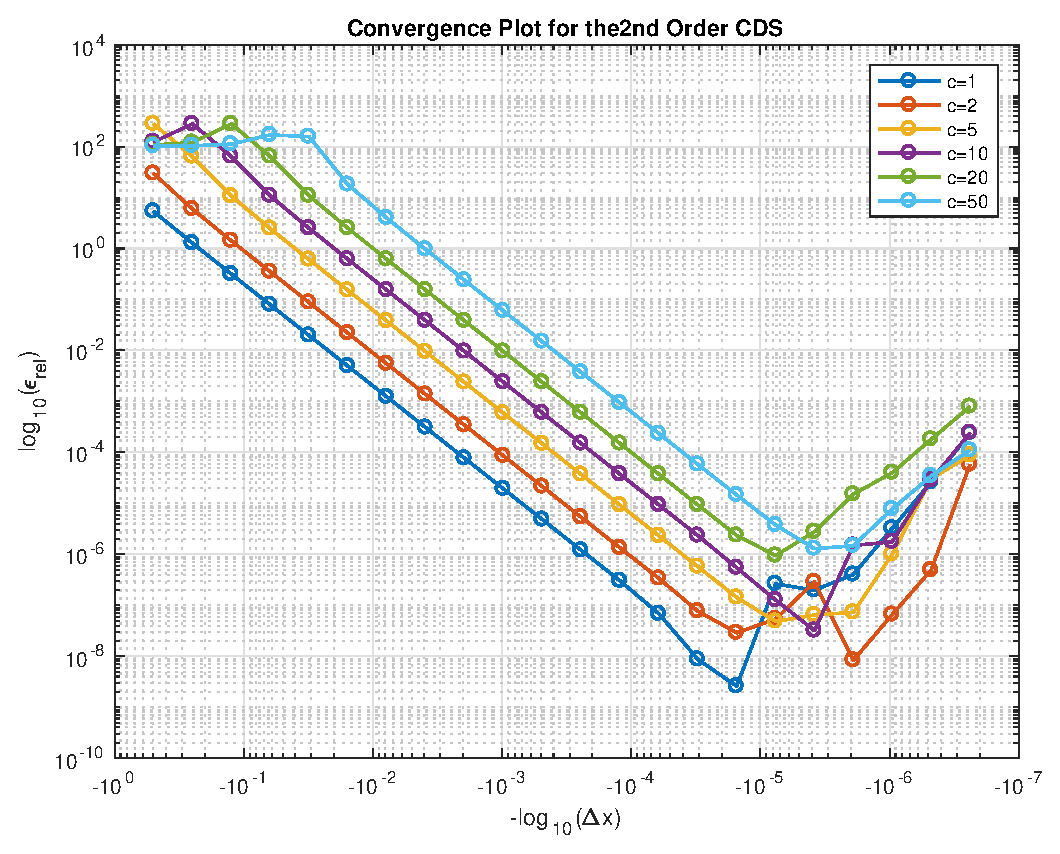
\includegraphics[width = 0.57\linewidth]{convergence_2nd_order_cds}
		\caption{Convergence Plot for 2nd-Order CDS FDM}	
	\end{center}
\end{figure}

\begin{table}[H]
	\input{roc_table_2nd_order_cds.tex}
	\caption{Rate of Convergence Values for 2nd-Order CDS FDM}	
\end{table}

\newpage

\subsection{4th-Order Central Difference Scheme First-Derivative Extraction}

\subsubsection{Derivation}

Developing the Taylor series for $u(x)$ in the vicinity of $x = 1$:
\begin{equation}
u_{N-1} = u_N - \Delta x u'_N + \frac{\Delta x^2}{2} u''_N - \frac{\Delta x^3}{6} u^{(3)}_N + \frac{\Delta x^4}{24} u^{(4)}_N + \mathcal{O}(\Delta x^5)
\end{equation}
Returning to the differential equation, rearranging for the second derivative, and taking two additional derivatives:
\begin{equation}
-u''(x)+cu'(x)=0
\end{equation}
\begin{equation}
u''(x)=cu'(x)
\end{equation}
\begin{equation}
u^{(3)}(x)=c^2u'(x)
\end{equation}
\begin{equation}
u^{(4)}(x)=c^3u'(x)
\end{equation}
Replacing the second-, third-, and fourth-derivative terms in the Taylor series expansion: 
\begin{equation}
u_{N-1} = u_N - \Delta x u'_N + \frac{c\Delta x^2}{2} u'_N - \frac{c^2\Delta x^3}{6} u'_N + \frac{c^3\Delta x^4}{24} u'_N + \mathcal{O}(\Delta x^5)
\end{equation}
\begin{equation}
\frac{u_{N}-u_{N-1}}{\Delta x} = \left(1 - \frac{c\Delta x}{2} + \frac{c^2\Delta x^2}{6} - \frac{c^3\Delta x^3}{24} \right)u'_N + \mathcal{O}(\Delta x^4)
\end{equation}
\begin{equation}
u'_N = \left(1 - \frac{c\Delta x}{2} + \frac{c^2\Delta x^2}{6} - \frac{c^3\Delta x^3}{24} \right)^{-1}\frac{u_{N}-u_{N-1}}{\Delta x} + \mathcal{O}(\Delta x^4)
\end{equation}
Applying the boundary condition $u(1) = u_N = 1$:
\begin{equation}
u'_N = \left(1 - \frac{c\Delta x}{2} + \frac{c^2\Delta x^2}{6} - \frac{c^3\Delta x^3}{24} \right)^{-1}\frac{1-u_{N-1}}{\Delta x} + \mathcal{O}(\Delta x^4)
\end{equation}

From this specific first-derivative formulation at the boundary $x = 1$ using the finite difference method, the approximation can be observed to be fourth-order ($\mathcal{O}(\Delta x^4)$).

\newpage

\subsubsection{Results}

Note: The quantity of interest for the 4th-order CDS FDM is extracted using the 4th-order first-derivative extraction - yielding the quantity of interest with an error of $\mathcal{O}(\Delta x^4)$.

\begin{figure}[H]
	\begin{center}
		\includegraphics[width = 0.57\linewidth]{convergence_4th_order_cds}
		\caption{Convergence Plot for 4th-Order CDS FDM}	
	\end{center}
\end{figure}

\begin{table}[H]
	\begin{tabular}{|c|c|c|c|c|c|c|}
\hline
\textbf{$\Delta x$}&\textbf{$\beta(c=1)$}&\textbf{$\beta(c=2)$}&\textbf{$\beta(c=5)$}&\textbf{$\beta(c=10)$}&\textbf{$\beta(c=20)$}&\textbf{$\beta(c=50)$}\\\hline
0.5000&4.1405&4.2684&5.7890&-0.5483&-0.0944&-0.0011\\\hline
0.2500&4.0749&4.1459&4.3454&5.7890&-0.5492&-0.0322\\\hline
0.1250&4.0389&4.0782&4.1839&4.3464&5.7889&-1.2503\\\hline
0.0625&4.0198&4.0407&4.1005&4.1847&4.3464&4.9348\\\hline
0.0312&4.0103&4.0208&4.0529&4.1010&4.1848&4.4625\\\hline
0.0156&4.0233&4.0112&4.0272&4.0532&4.1010&4.2233\\\hline
0.0078&6.7476&4.0609&4.0142&4.0274&4.0532&4.1232\\\hline
0.0039&-4.5113&3.7287&4.0311&4.0143&4.0274&4.0657\\\hline
0.0020&-1.9775&-2.9750&7.5728&4.0329&4.0143&4.0340\\\hline
0.0010&-1.9979&-1.9307&-5.7027&6.5530&4.0323&4.0175\\\hline
0.0005&-1.9992&-1.9571&-2.0388&-4.7944&7.1048&4.0140\\\hline
0.0002&-1.9781&-2.0422&-1.9624&-2.0272&-5.2245&4.0011\\\hline
0.0001&-2.0174&-1.9810&-2.0355&-1.9977&-2.0860&4.1025\\\hline
0.0001&-2.0013&-2.0205&-1.9915&-1.9714&-2.0585&3.2178\\\hline
0.0000&-1.9917&-1.9825&-2.0030&-2.0012&-1.7842&-1.8639\\\hline
0.0000&-2.0022&-1.9949&-1.9876&-1.8558&-2.5308&-0.8759\\\hline
0.0000&-2.0021&-2.0102&-2.0060&-2.0094&-2.5697&-0.7555\\\hline
0.0000&-1.9991&-1.9939&-1.9989&-2.0981&-1.3343&-14.7059\\\hline
0.0000&-1.9985&-1.9998&-2.0049&-2.0182&-2.4899&-1.9214\\\hline
0.0000&-1.9986&-1.9998&-1.9684&-2.0010&1.2231&13.4265\\\hline
0.0000&-1.9973&-1.9968&-1.9979&-1.8221&-4.4135&-17.3388\\\hline
\end{tabular}

	\caption{Rate of Convergence Values for 4th-Order CDS FDM}	
\end{table}

\newpage

\subsection{1st-Order Upwind Scheme First-Derivative Extraction}

\subsubsection{Derivation}

Developing the Taylor series for $u(x)$ in the vicinity of $x = 1$:
\begin{equation}
u_{N-1} = u_N - \Delta x u'_N + \mathcal{O}(\Delta x^2)
\end{equation}
Rearranging terms to solve for $u'_N$:
\begin{equation}
u'_N = \frac{u_N - u_{N-1}}{\Delta x} + \mathcal{O}(\Delta x)
\end{equation}
Applying the boundary condition $u(1) = u_N = 1$:
\begin{equation}
u'_N = \frac{1 - u_{N-1}}{\Delta x} + \mathcal{O}(\Delta x)
\end{equation}

From this specific first-derivative formulation at the boundary $x = 1$ using the finite difference method, the approximation can be observed to be first-order ($\mathcal{O}(\Delta x)$).

\newpage

\subsubsection{Results}

Note: The quantity of interest for the 1st-order US FDM is extracted using the 1st-order first-derivative extraction - yielding the quantity of interest with an error of $\mathcal{O}(\Delta x)$.

\begin{figure}[H]
	\begin{center}
		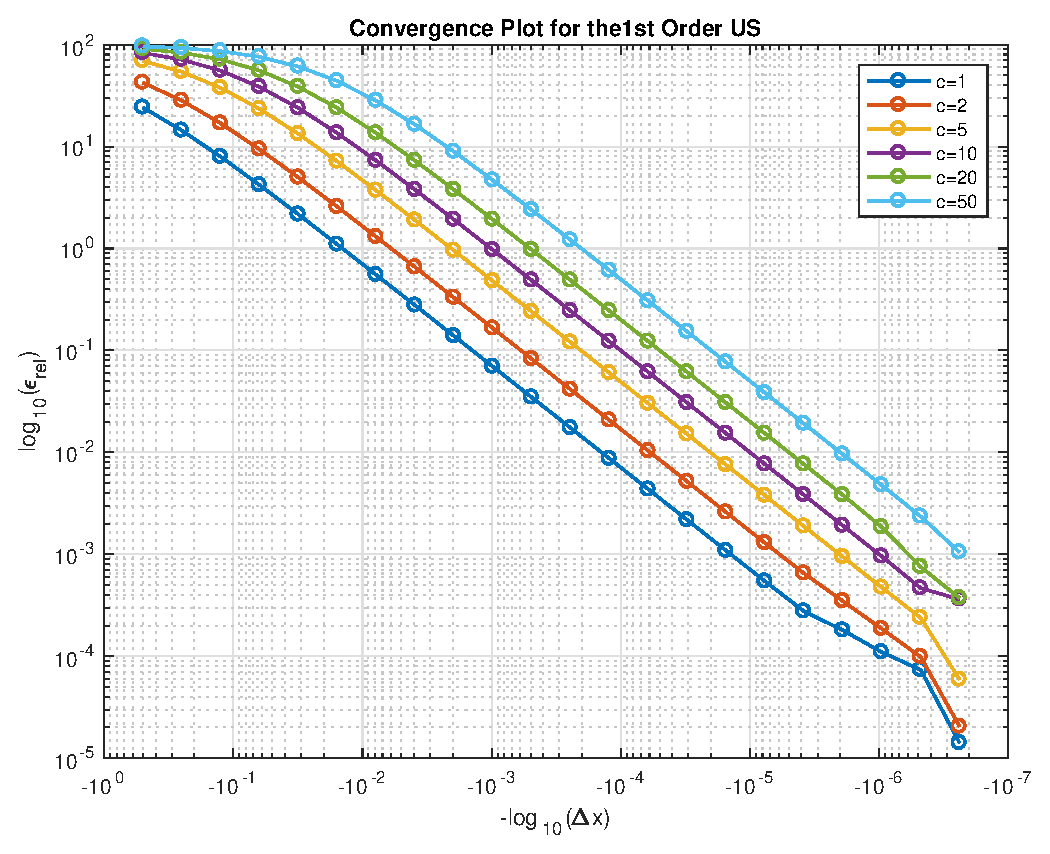
\includegraphics[width = 0.56\linewidth]{convergence_1st_order_us}
		\caption{Convergence Plot 1st-Order US FDM}	
	\end{center}
\end{figure}

\begin{table}[H]
	\begin{tabular}{|c|c|c|c|c|c|c|}
\hline
\textbf{$\Delta x$}&\textbf{$\beta(c=1)$}&\textbf{$\beta(c=2)$}&\textbf{$\beta(c=5)$}&\textbf{$\beta(c=10)$}&\textbf{$\beta(c=20)$}&\textbf{$\beta(c=50)$}\\\hline
0.5000&0.7510&0.5886&0.3540&0.2180&0.1246&0.0544\\\hline
0.2500&0.8560&0.7385&0.5242&0.3604&0.2222&0.1031\\\hline
0.1250&0.9218&0.8486&0.6880&0.5297&0.3625&0.1864\\\hline
0.0625&0.9592&0.9178&0.8150&0.6916&0.5305&0.3132\\\hline
0.0312&0.9791&0.9570&0.8980&0.8170&0.6919&0.4753\\\hline
0.0156&0.9894&0.9780&0.9462&0.8990&0.8171&0.6428\\\hline
0.0078&0.9947&0.9889&0.9723&0.9467&0.8991&0.7817\\\hline
0.0039&0.9973&0.9944&0.9860&0.9726&0.9468&0.8770\\\hline
0.0020&0.9987&0.9972&0.9929&0.9861&0.9726&0.9344\\\hline
0.0010&0.9993&0.9986&0.9965&0.9930&0.9861&0.9660\\\hline
0.0005&0.9997&0.9993&0.9982&0.9965&0.9930&0.9827\\\hline
0.0002&0.9998&0.9996&0.9991&0.9982&0.9965&0.9913\\\hline
0.0001&0.9999&0.9998&0.9996&0.9991&0.9982&0.9956\\\hline
0.0001&1.0000&0.9999&0.9998&0.9996&0.9991&0.9978\\\hline
0.0000&1.0001&1.0000&0.9999&0.9998&0.9996&0.9989\\\hline
0.0000&0.9985&0.9998&0.9999&0.9999&0.9998&0.9995\\\hline
0.0000&0.9748&0.9855&0.9980&0.9999&1.0004&0.9998\\\hline
0.0000&0.6167&0.9060&0.9954&1.0000&1.0044&1.0001\\\hline
0.0000&0.7135&0.9028&0.9956&1.0010&1.0418&1.0019\\\hline
0.0000&0.5778&0.9135&0.9886&1.0342&1.2966&1.0190\\\hline
0.0000&2.3818&2.2734&2.0125&0.3676&1.0159&1.1684\\\hline
\end{tabular}

	\caption{Rate of Convergence Values for 1st-Order US FDM}	
\end{table}

\subsection{Comparison of 2nd-Order CDS, 4th-Order CDS, and 1st-Order US Finite Difference Methods}

\begin{figure}[H]
	\begin{center}
		\includegraphics[width=0.46\linewidth]{convergence_c_1}
		\includegraphics[width=0.46\linewidth]{convergence_c_2}
		\includegraphics[width=0.46\linewidth]{convergence_c_5}
		\includegraphics[width=0.46\linewidth]{convergence_c_10}
		\includegraphics[width=0.46\linewidth]{convergence_c_20}
		\includegraphics[width=0.46\linewidth]{convergence_c_50}
	\end{center}
\end{figure}

\subsection{Discussion}

As was explored earlier, the composite order of the solution to the boundary-value problem is dependent on the lowest-order method used across the entire solution -- in this case, the lowest-order method of the finite difference method and the extraction method. Thus, the extraction method was developed to be equal to the highest-order method used, so that the rates of convergence could be easily seen.

For the 2nd-order CDS FDM, the rate of convergence is shown to be approximately 2 (\textbf{quadratic convergence}), which is predicted by order of the error calculations. At small mesh sizes, the error begins to increase as a function of increasing mesh size -- typical of such small mesh sizes. We can see that a number of simulations, for example, those at $c=50$ at the coarsest mesh sizes actually have more than 100\% relative error. This is due to the violation of the Peclet condition and earlier described unstable oscillations that develop in the scheme. These oscillations and their errors disappear once the mesh size is sufficiently small that the Peclet condition is satified.

For the 4th-order CDS FDM, the rate of convergence is shown to be approximately 4 and sometimes a little more than 4 (\textbf{quartic to superquartic convergence}), which is predicted by order of the error calculations. At moderately small mesh sizes, the error begins to increase as a function of increasing mesh size -- typical of such small mesh sizes. However, compared to the 2nd-order CDS FDM, the onset of the error increase is much earlier - this is because of the increased accuracy provided earlier on for coarser meshes. We also observe some odd trends for the case $c=50$.

For the 1st-order US FDM, the rate of convergence is shown to be approximately 1 and sometimes a little less than 1 (\textbf{sublinear to linear convergence}), which is predicted by order of the error calculations. Even at very small mesh sizes, the error never increases as a function of increasing mesh size -- though at the smallest mesh size tested, there appears to be the development of the trend reversal, as seen for other methods.

\vspace{30 pt}

A simultaneous comparison of all of the methods for various values of $c$ proves that:

\begin{itemize}
	\item the second-order central difference scheme finite difference method is quadratically convergent
	\item the fourth-order central difference scheme finite difference method is quartically convergent
	\item the first-order upwind scheme finite difference method is linearly convergent
\end{itemize}

\newpage

\appendix

\section{$u(x)$ v. $u_{exact}(x)$ Tables}

Error tables are included here up to a mesh spacing of $\Delta x = \left(\frac{1}{2}\right)^5$, but are available for all mesh spacings through the MATLAB code.

\subsection{2nd-Order CDS FDM}

\begin{tabular}{|c|c|c|c|}
\hline
\textbf{$x$}&\textbf{$u(x)$}&\textbf{$\bar{u}(x)$}&\textbf{$\epsilon_{rel}$}\\\hline
0.00e+00&0.00e+00&0.00e+00&NaN\\\hline
5.00e-01&-5.75e+00&1.39e-11&4.14e+13\\\hline
1.00e+00&1.00e+00&1.00e+00&0.00e+00\\\hline
\end{tabular}

\begin{tabular}{|c|c|c|c|}
\hline
\textbf{$x$}&\textbf{$u(x)$}&\textbf{$\bar{u}(x)$}&\textbf{$\epsilon_{rel}$}\\\hline
0.00e+00&-6.13e-17&0.00e+00&Inf\\\hline
2.50e-01&-9.03e-01&5.18e-17&1.74e+18\\\hline
5.00e-01&3.44e-01&1.39e-11&2.48e+12\\\hline
7.50e-01&-1.38e+00&3.73e-06&3.70e+07\\\hline
1.00e+00&1.00e+00&1.00e+00&0.00e+00\\\hline
\end{tabular}

\newline
\begin{tabular}{|c|c|c|c|}
\hline
\textbf{$x$}&\textbf{$u(x)$}&\textbf{$\bar{u}(x)$}&\textbf{$\epsilon_{rel}$}\\\hline
0.00e+00&2.61e-17&0.00e+00&Inf\\\hline
1.25e-01&-1.47e-02&9.97e-20&1.47e+19\\\hline
2.50e-01&1.38e-02&5.18e-17&2.67e+16\\\hline
3.75e-01&-4.14e-02&2.68e-14&1.55e+14\\\hline
5.00e-01&6.58e-02&1.39e-11&4.74e+11\\\hline
6.25e-01&-1.42e-01&7.19e-09&1.98e+09\\\hline
7.50e-01&2.62e-01&3.73e-06&7.02e+06\\\hline
8.75e-01&-5.23e-01&1.93e-03&2.72e+04\\\hline
1.00e+00&1.00e+00&1.00e+00&0.00e+00\\\hline
\end{tabular}

\begin{tabular}{|c|c|c|c|}
\hline
\textbf{$x$}&\textbf{$u(x)$}&\textbf{$\bar{u}(x)$}&\textbf{$\epsilon_{rel}$}\\\hline
0.00e+00&7.93e-18&0.00e+00&Inf\\\hline
6.25e-02&-1.61e-10&4.20e-21&3.85e+12\\\hline
1.25e-01&5.74e-10&9.97e-20&5.76e+11\\\hline
1.88e-01&-2.78e-09&2.27e-18&1.22e+11\\\hline
2.50e-01&1.25e-08&5.18e-17&2.41e+10\\\hline
3.12e-01&-5.71e-08&1.18e-15&4.84e+09\\\hline
3.75e-01&2.60e-07&2.68e-14&9.69e+08\\\hline
4.38e-01&-1.18e-06&6.10e-13&1.94e+08\\\hline
5.00e-01&5.39e-06&1.39e-11&3.88e+07\\\hline
5.62e-01&-2.46e-05&3.16e-10&7.77e+06\\\hline
6.25e-01&1.12e-04&7.19e-09&1.56e+06\\\hline
6.88e-01&-5.10e-04&1.64e-07&3.11e+05\\\hline
7.50e-01&2.32e-03&3.73e-06&6.22e+04\\\hline
8.12e-01&-1.06e-02&8.48e-05&1.26e+04\\\hline
8.75e-01&4.82e-02&1.93e-03&2.40e+03\\\hline
9.38e-01&-2.20e-01&4.39e-02&6.00e+02\\\hline
1.00e+00&1.00e+00&1.00e+00&0.00e+00\\\hline
\end{tabular}

\newline
\begin{tabular}{|c|c|c|c|}
\hline
\textbf{$x$}&\textbf{$u(x)$}&\textbf{$\bar{u}(x)$}&\textbf{$\epsilon_{rel}$}\\\hline
0.00e+00&-8.12e-18&0.00e+00&Inf\\\hline
3.12e-02&-8.12e-18&7.27e-22&1.12e+06\\\hline
6.25e-02&-8.12e-18&4.20e-21&1.94e+05\\\hline
9.38e-02&-8.12e-18&2.07e-20&3.92e+04\\\hline
1.25e-01&-8.12e-18&9.97e-20&8.24e+03\\\hline
1.56e-01&-8.12e-18&4.76e-19&1.80e+03\\\hline
1.88e-01&-8.12e-18&2.27e-18&4.57e+02\\\hline
2.19e-01&-8.12e-18&1.08e-17&1.75e+02\\\hline
2.50e-01&-8.12e-18&5.18e-17&1.16e+02\\\hline
2.81e-01&-8.12e-18&2.47e-16&1.03e+02\\\hline
3.12e-01&-8.11e-18&1.18e-15&1.01e+02\\\hline
3.44e-01&-8.04e-18&5.62e-15&1.00e+02\\\hline
3.75e-01&-7.51e-18&2.68e-14&1.00e+02\\\hline
4.06e-01&-3.16e-18&1.28e-13&1.00e+02\\\hline
4.38e-01&3.22e-17&6.10e-13&1.00e+02\\\hline
4.69e-01&3.21e-16&2.91e-12&1.00e+02\\\hline
5.00e-01&2.67e-15&1.39e-11&1.00e+02\\\hline
5.31e-01&2.18e-14&6.63e-11&1.00e+02\\\hline
5.62e-01&1.77e-13&3.16e-10&9.99e+01\\\hline
5.94e-01&1.45e-12&1.51e-09&9.99e+01\\\hline
6.25e-01&1.18e-11&7.19e-09&9.98e+01\\\hline
6.56e-01&9.58e-11&3.43e-08&9.97e+01\\\hline
6.88e-01&7.80e-10&1.64e-07&9.95e+01\\\hline
7.19e-01&6.35e-09&7.81e-07&9.92e+01\\\hline
7.50e-01&5.17e-08&3.73e-06&9.86e+01\\\hline
7.81e-01&4.21e-07&1.78e-05&9.76e+01\\\hline
8.12e-01&3.43e-06&8.48e-05&9.60e+01\\\hline
8.44e-01&2.79e-05&4.05e-04&9.31e+01\\\hline
8.75e-01&2.27e-04&1.93e-03&8.82e+01\\\hline
9.06e-01&1.85e-03&9.21e-03&7.99e+01\\\hline
9.38e-01&1.51e-02&4.39e-02&6.57e+01\\\hline
9.69e-01&1.23e-01&2.10e-01&4.14e+01\\\hline
1.00e+00&1.00e+00&1.00e+00&0.00e+00\\\hline
\end{tabular}


\newpage

\subsection{4th-Order CDS FDM}

\begin{tabular}{|c|c|c|c|}
\hline
\textbf{$x$}&\textbf{$u(x)$}&\textbf{$\bar{u}(x)$}&\textbf{$\epsilon_{rel}$}\\\hline
0.00e+00&1.09e-18&0.00e+00&Inf\\\hline
5.00e-01&3.82e-01&1.39e-11&2.75e+12\\\hline
1.00e+00&1.00e+00&1.00e+00&0.00e+00\\\hline
\end{tabular}

\begin{tabular}{|c|c|c|c|}
\hline
\textbf{$x$}&\textbf{$u(x)$}&\textbf{$\bar{u}(x)$}&\textbf{$\epsilon_{rel}$}\\\hline
0.00e+00&1.26e-17&0.00e+00&Inf\\\hline
2.50e-01&3.55e-02&5.18e-17&6.86e+16\\\hline
5.00e-01&1.28e-01&1.39e-11&9.23e+11\\\hline
7.50e-01&3.70e-01&3.73e-06&9.92e+06\\\hline
1.00e+00&1.00e+00&1.00e+00&0.00e+00\\\hline
\end{tabular}

\newline
\begin{tabular}{|c|c|c|c|}
\hline
\textbf{$x$}&\textbf{$u(x)$}&\textbf{$\bar{u}(x)$}&\textbf{$\epsilon_{rel}$}\\\hline
0.00e+00&-1.47e-17&0.00e+00&Inf\\\hline
1.25e-01&1.67e-06&9.97e-20&1.68e+15\\\hline
2.50e-01&1.26e-05&5.18e-17&2.43e+13\\\hline
3.75e-01&8.39e-05&2.68e-14&3.13e+11\\\hline
5.00e-01&5.50e-04&1.39e-11&3.96e+09\\\hline
6.25e-01&3.59e-03&7.19e-09&4.99e+07\\\hline
7.50e-01&2.35e-02&3.73e-06&6.29e+05\\\hline
8.75e-01&1.53e-01&1.93e-03&7.83e+03\\\hline
1.00e+00&1.00e+00&1.00e+00&0.00e+00\\\hline
\end{tabular}

\begin{tabular}{|c|c|c|c|}
\hline
\textbf{$x$}&\textbf{$u(x)$}&\textbf{$\bar{u}(x)$}&\textbf{$\epsilon_{rel}$}\\\hline
0.00e+00&3.68e-18&0.00e+00&Inf\\\hline
6.25e-02&1.47e-17&4.20e-21&3.51e+05\\\hline
1.25e-01&1.63e-16&9.97e-20&1.63e+05\\\hline
1.88e-01&2.15e-15&2.27e-18&9.47e+04\\\hline
2.50e-01&2.89e-14&5.18e-17&5.58e+04\\\hline
3.12e-01&3.88e-13&1.18e-15&3.29e+04\\\hline
3.75e-01&5.22e-12&2.68e-14&1.94e+04\\\hline
4.38e-01&7.01e-11&6.10e-13&1.14e+04\\\hline
5.00e-01&9.42e-10&1.39e-11&6.68e+03\\\hline
5.62e-01&1.27e-08&3.16e-10&3.90e+03\\\hline
6.25e-01&1.70e-07&7.19e-09&2.26e+03\\\hline
6.88e-01&2.28e-06&1.64e-07&1.30e+03\\\hline
7.50e-01&3.07e-05&3.73e-06&7.24e+02\\\hline
8.12e-01&4.12e-04&8.48e-05&3.86e+02\\\hline
8.75e-01&5.54e-03&1.93e-03&1.87e+02\\\hline
9.38e-01&7.44e-02&4.39e-02&6.94e+01\\\hline
1.00e+00&1.00e+00&1.00e+00&0.00e+00\\\hline
\end{tabular}

\newline
\begin{tabular}{|c|c|c|c|}
\hline
\textbf{$x$}&\textbf{$u(x)$}&\textbf{$\bar{u}(x)$}&\textbf{$\epsilon_{rel}$}\\\hline
0.00e+00&2.03e-17&0.00e+00&Inf\\\hline
3.12e-02&2.03e-17&7.27e-22&2.79e+06\\\hline
6.25e-02&2.03e-17&4.20e-21&4.83e+05\\\hline
9.38e-02&2.03e-17&2.07e-20&9.77e+04\\\hline
1.25e-01&2.04e-17&9.97e-20&2.04e+04\\\hline
1.56e-01&2.10e-17&4.76e-19&4.30e+03\\\hline
1.88e-01&2.36e-17&2.27e-18&9.38e+02\\\hline
2.19e-01&3.60e-17&1.08e-17&2.31e+02\\\hline
2.50e-01&9.40e-17&5.18e-17&8.17e+01\\\hline
2.81e-01&3.67e-16&2.47e-16&4.86e+01\\\hline
3.12e-01&1.65e-15&1.18e-15&4.01e+01\\\hline
3.44e-01&7.68e-15&5.62e-15&3.67e+01\\\hline
3.75e-01&3.60e-14&2.68e-14&3.44e+01\\\hline
4.06e-01&1.69e-13&1.28e-13&3.24e+01\\\hline
4.38e-01&7.96e-13&6.10e-13&3.04e+01\\\hline
4.69e-01&3.74e-12&2.91e-12&2.85e+01\\\hline
5.00e-01&1.76e-11&1.39e-11&2.66e+01\\\hline
5.31e-01&8.27e-11&6.63e-11&2.48e+01\\\hline
5.62e-01&3.89e-10&3.16e-10&2.29e+01\\\hline
5.94e-01&1.83e-09&1.51e-09&2.11e+01\\\hline
6.25e-01&8.59e-09&7.19e-09&1.94e+01\\\hline
6.56e-01&4.04e-08&3.43e-08&1.76e+01\\\hline
6.88e-01&1.90e-07&1.64e-07&1.59e+01\\\hline
7.19e-01&8.92e-07&7.81e-07&1.42e+01\\\hline
7.50e-01&4.19e-06&3.73e-06&1.25e+01\\\hline
7.81e-01&1.97e-05&1.78e-05&1.09e+01\\\hline
8.12e-01&9.27e-05&8.48e-05&9.26e+00\\\hline
8.44e-01&4.36e-04&4.05e-04&7.66e+00\\\hline
8.75e-01&2.05e-03&1.93e-03&6.08e+00\\\hline
9.06e-01&9.63e-03&9.21e-03&4.53e+00\\\hline
9.38e-01&4.53e-02&4.39e-02&3.00e+00\\\hline
9.69e-01&2.13e-01&2.10e-01&1.49e+00\\\hline
1.00e+00&1.00e+00&1.00e+00&0.00e+00\\\hline
\end{tabular}


\newpage

\subsection{1st-Order US FDM}

\begin{tabular}{|c|c|c|c|}
\hline
\textbf{$x$}&\textbf{$u(x)$}&\textbf{$\bar{u}(x)$}&\textbf{$\epsilon_{rel}$}\\\hline
0.00e+00&-2.14e-18&0.00e+00&Inf\\\hline
5.00e-01&3.70e-02&1.39e-11&2.67e+11\\\hline
1.00e+00&1.00e+00&1.00e+00&0.00e+00\\\hline
\end{tabular}

\begin{tabular}{|c|c|c|c|}
\hline
\textbf{$x$}&\textbf{$u(x)$}&\textbf{$\bar{u}(x)$}&\textbf{$\epsilon_{rel}$}\\\hline
0.00e+00&-6.91e-18&0.00e+00&Inf\\\hline
2.50e-01&3.76e-04&5.18e-17&7.27e+14\\\hline
5.00e-01&5.46e-03&1.39e-11&3.93e+10\\\hline
7.50e-01&7.40e-02&3.73e-06&1.99e+06\\\hline
1.00e+00&1.00e+00&1.00e+00&0.00e+00\\\hline
\end{tabular}

\newline
\begin{tabular}{|c|c|c|c|}
\hline
\textbf{$x$}&\textbf{$u(x)$}&\textbf{$\bar{u}(x)$}&\textbf{$\epsilon_{rel}$}\\\hline
0.00e+00&-5.15e-18&0.00e+00&Inf\\\hline
1.25e-01&8.19e-07&9.97e-20&8.21e+14\\\hline
2.50e-01&6.76e-06&5.18e-17&1.31e+13\\\hline
3.75e-01&4.98e-05&2.68e-14&1.86e+11\\\hline
5.00e-01&3.62e-04&1.39e-11&2.61e+09\\\hline
6.25e-01&2.62e-03&7.19e-09&3.65e+07\\\hline
7.50e-01&1.90e-02&3.73e-06&5.10e+05\\\hline
8.75e-01&1.38e-01&1.93e-03&7.04e+03\\\hline
1.00e+00&1.00e+00&1.00e+00&0.00e+00\\\hline
\end{tabular}

\begin{tabular}{|c|c|c|c|}
\hline
\textbf{$x$}&\textbf{$u(x)$}&\textbf{$\bar{u}(x)$}&\textbf{$\epsilon_{rel}$}\\\hline
0.00e+00&-9.76e-18&0.00e+00&Inf\\\hline
6.25e-02&4.45e-10&4.20e-21&1.06e+13\\\hline
1.25e-01&2.28e-09&9.97e-20&2.29e+12\\\hline
1.88e-01&9.85e-09&2.27e-18&4.33e+11\\\hline
2.50e-01&4.11e-08&5.18e-17&7.93e+10\\\hline
3.12e-01&1.70e-07&1.18e-15&1.44e+10\\\hline
3.75e-01&7.01e-07&2.68e-14&2.61e+09\\\hline
4.38e-01&2.89e-06&6.10e-13&4.74e+08\\\hline
5.00e-01&1.19e-05&1.39e-11&8.59e+07\\\hline
5.62e-01&4.92e-05&3.16e-10&1.56e+07\\\hline
6.25e-01&2.03e-04&7.19e-09&2.82e+06\\\hline
6.88e-01&8.37e-04&1.64e-07&5.11e+05\\\hline
7.50e-01&3.45e-03&3.73e-06&9.26e+04\\\hline
8.12e-01&1.42e-02&8.48e-05&1.67e+04\\\hline
8.75e-01&5.88e-02&1.93e-03&2.94e+03\\\hline
9.38e-01&2.42e-01&4.39e-02&4.52e+02\\\hline
1.00e+00&1.00e+00&1.00e+00&0.00e+00\\\hline
\end{tabular}

\newline
\begin{tabular}{|c|c|c|c|}
\hline
\textbf{$x$}&\textbf{$u(x)$}&\textbf{$\bar{u}(x)$}&\textbf{$\epsilon_{rel}$}\\\hline
0.00e+00&5.76e-17&0.00e+00&Inf\\\hline
3.12e-02&1.31e-13&7.27e-22&1.80e+10\\\hline
6.25e-02&4.66e-13&4.20e-21&1.11e+10\\\hline
9.38e-02&1.32e-12&2.07e-20&6.38e+09\\\hline
1.25e-01&3.53e-12&9.97e-20&3.54e+09\\\hline
1.56e-01&9.16e-12&4.76e-19&1.92e+09\\\hline
1.88e-01&2.36e-11&2.27e-18&1.04e+09\\\hline
2.19e-01&6.06e-11&1.08e-17&5.59e+08\\\hline
2.50e-01&1.56e-10&5.18e-17&3.01e+08\\\hline
2.81e-01&3.99e-10&2.47e-16&1.61e+08\\\hline
3.12e-01&1.02e-09&1.18e-15&8.67e+07\\\hline
3.44e-01&2.62e-09&5.62e-15&4.66e+07\\\hline
3.75e-01&6.71e-09&2.68e-14&2.50e+07\\\hline
4.06e-01&1.72e-08&1.28e-13&1.34e+07\\\hline
4.38e-01&4.41e-08&6.10e-13&7.22e+06\\\hline
4.69e-01&1.13e-07&2.91e-12&3.88e+06\\\hline
5.00e-01&2.89e-07&1.39e-11&2.08e+06\\\hline
5.31e-01&7.41e-07&6.63e-11&1.12e+06\\\hline
5.62e-01&1.90e-06&3.16e-10&6.01e+05\\\hline
5.94e-01&4.87e-06&1.51e-09&3.23e+05\\\hline
6.25e-01&1.25e-05&7.19e-09&1.73e+05\\\hline
6.56e-01&3.20e-05&3.43e-08&9.30e+04\\\hline
6.88e-01&8.19e-05&1.64e-07&4.99e+04\\\hline
7.19e-01&2.10e-04&7.81e-07&2.68e+04\\\hline
7.50e-01&5.38e-04&3.73e-06&1.43e+04\\\hline
7.81e-01&1.38e-03&1.78e-05&7.65e+03\\\hline
8.12e-01&3.53e-03&8.48e-05&4.06e+03\\\hline
8.44e-01&9.05e-03&4.05e-04&2.14e+03\\\hline
8.75e-01&2.32e-02&1.93e-03&1.10e+03\\\hline
9.06e-01&5.94e-02&9.21e-03&5.45e+02\\\hline
9.38e-01&1.52e-01&4.39e-02&2.47e+02\\\hline
9.69e-01&3.90e-01&2.10e-01&8.62e+01\\\hline
1.00e+00&1.00e+00&1.00e+00&0.00e+00\\\hline
\end{tabular}


\newpage

\section{MATLAB Code}

\begin{lstlisting}
clear all; close all; clc

%% Initial Conditions

plotGen     = false;
plotSave    = false;
tableSave   = false;
tableSave2  = false;
tableSave3  = false;

odeType = '1st Order US';
%odeType = '2nd Order CDS';
%odeType = '4th Order CDS';

odeString = '1st_Order_US';

mesh.order = 1:22;
mesh.dx = 0.5.^mesh.order;

rowID = 0;

%% Boundary Value Problem Solution

for c = [50]

	rowID = rowID + 1;
	colID = 0;

	if plotGen

		fig1 = figure(1);
		xlabel('x');    ylabel('u(x)');
		grid on;        grid minor;
		box on;         hold on;
		set(gcf, 'Position', [1 1 624 550])

		if strcmpi(odeType, '2nd Order CDS')
			titleString = strcat('2nd Order CDS FDM for c=', num2str(c));
		elseif strcmpi(odeType, '4th Order CDS')
			titleString = strcat('4th Order CDS FDM for c=', num2str(c));
		elseif strcmpi(odeType, '1st Order US')
			titleString = strcat('1st Order US FDM for c=', num2str(c));
		end
	
		title(titleString)
		
		fig2 = figure(2);
		xlabel('x');    ylabel('\epsilon_{rel}');
		grid on;        grid minor;
		box on;         hold on;
		set(gcf, 'Position', [1 1 624 550])
		
		title(titleString)
	
	end

	for dx = mesh.dx
	
		nx = 1 / dx + 1;
		x = linspace(0, 1, nx);
		b = zeros(nx, 1);
		colID = colID + 1;
	
		if strcmpi(odeType, '2nd Order CDS')
			alpha = -1 - c*dx/2;
			beta = 2;
			gamma = -1 + c*dx/2;
		elseif strcmpi(odeType, '4th Order CDS')
			alpha = -1 - c*dx/2 - c^2*dx^2/12;
			beta = 2 + c^2*dx^2/6;
			gamma = -1 + c*dx/2 - c^2*dx^2/12;
		elseif strcmpi(odeType, '1st Order US')
			alpha = -1 - c*dx;
			beta = 2 + c*dx;
			gamma = -1;
		end
	
		A = gallery('tridiag', nx, alpha, beta, gamma);
		
		A(1, 1) = 1;    A(1, 2) = 0;        b(1) = 0;
		A(nx, nx) = 1;  A(nx, nx-1) = 0;    b(nx) = 1;
		b(2:nx-1) = 0;
		
		u = A\b;
	
		if plotGen && dx >= mesh.dx(8)
		
			figure(1)
			plot(x, u, 'linewidth', 1)
		
		end
	
		if strcmpi(odeType, '2nd Order CDS')
			dudx.fdm(rowID, colID) = (1 -c*dx/2)^-1 * (1 - u(end-1)) / dx;
		elseif strcmpi(odeType, '4th Order CDS')
			dudx.fdm(rowID, colID) = (1 -c*dx/2 + c^2*dx^2/6 - c^3*dx^3/24)^-1 * ...
			(1 - u(end-1)) / dx;
		elseif strcmpi(odeType, '1st Order US')
			dudx.fdm(rowID, colID) = (1 - u(end-1)) / dx;
		end
	
		ux.exact = (exp(c*x) - 1) / (exp(c) - 1);
		dudx.exact(rowID, colID) = c*exp(c) / (exp(c) - 1);
	
		if plotGen && dx >= mesh.dx(8)
		
			figure(2)
			plot(x(2:end-1), abs(ux.exact(2:end-1)'-u(2:end-1)) ./ ...
			abs(ux.exact(2:end-1)')*100, 'o-')
		
		end
	
		if tableSave2 && dx >= mesh.dx(5)
		
			colLabels = {'$x$', '$u(x)$', '$\bar{u}(x)$', '$\epsilon_{rel}$'};
		
			matrix2latex([x' u ux.exact' (abs(ux.exact'-u)./abs(ux.exact')*100)], ...
			strcat('pointwise_error_table_dx_', num2str(nx), '_', lower(odeString), '.tex'), ...
			'columnLabels', colLabels, 'alignment', 'c', 'format', '%1.2e')
		
		end
	
	end

	if plotGen
	
		figure(1)
		
		fplot(@(x) (exp(c*x)-1)/(exp(c) - 1), [0 1], '-k', 'linewidth', 1.5)
		
		legend('\Deltax = (1/2)^1', '\Deltax = (1/2)^2', '\Deltax = (1/2)^3', ...
		'\Deltax = (1/2)^4', '\Deltax = (1/2)^5', '\Deltax = (1/2)^6', ...
		'\Deltax = (1/2)^7', '\Deltax = (1/2)^8', 'Analytical Solution', ...
		'location', 'eastoutside')
	
		drawnow
		
		figure(2)
		
		legend('\Deltax = (1/2)^1', '\Deltax = (1/2)^2', '\Deltax = (1/2)^3', ...
		'\Deltax = (1/2)^4', '\Deltax = (1/2)^5', '\Deltax = (1/2)^6', ...
		'\Deltax = (1/2)^7', '\Deltax = (1/2)^8', 'location', 'eastoutside')
		set(gca, 'YScale', 'log')
		
		drawnow
	
		if plotSave
		
			figure(1)
			figureString = strcat('solution_', lower(odeString), '_c_', num2str(c));
			saveas(gcf, figureString, 'epsc')
			
			figure(2)
			figureString = strcat('pointwise_error_', lower(odeString), '_c_', num2str(c));
			saveas(gcf, figureString, 'epsc')
			
			close gcf;  close gcf
		
		end
	
	end

end


%% Convergence Analysis

relError = abs(dudx.exact-dudx.fdm) ./ abs(dudx.exact) * 100;

if plotGen

	figure
	xlabel('-log_{10}(\Deltax)');   ylabel('log_{10}(\epsilon_{rel})');
	grid on;                        grid minor;
	box on;                         hold on;
	
	for kID = 1:6
		loglog(-mesh.dx, relError(kID, :), '-o', 'linewidth', 1.25);
	end
	
	title(strcat('Convergence Plot for the ', odeType))
	legend('c=1', 'c=2', 'c=5', 'c=10', 'c=20', 'c=50')
	set(gca, 'XScale', 'log');  set(gca, 'YScale', 'log');
	drawnow

	if plotSave
	
		figureString = strcat('convergence_', lower(odeString));
		saveas(gcf, figureString, 'epsc')
		close gcf
	
	end

end

%% Rate of Convergence Analysis

logRelError = log10(relError);

for kID = 1:6

	for rocID = 1:length(logRelError) - 1
		roc(kID, rocID) = (logRelError(kID, rocID+1) - logRelError(kID, rocID)) / -log10(2);
	end

end

colLabels = {'$\Delta x$', '$\beta(c=1)$', '$\beta(c=2)$', '$\beta(c=5)$', ...
'$\beta(c=10)$', '$\beta(c=20)$', '$\beta(c=50)$'};

if tableSave

	matrix2latex([mesh.dx(1:end-1)' roc'], strcat('roc_table_', lower(odeString), '.tex'), ...
	'columnLabels', colLabels, 'alignment', 'c', 'format', '%5.4f')

end

colLabels1 = {'$\Delta x$', '$u''_{c=1}(1)$', '$u''_{c=2}(1)$', '$u''_{c=5}(1)$', ...
'$\bar{u}''_{c=1}(1)$', '$\bar{u}''_{c=2}(1)$', '$\bar{u}''_{c=5}(1)$', ...
'$\epsilon''_{rel,c=1}$', '$\epsilon''_{rel,c=2}$', '$\epsilon''_{rel,c=5}$'};
colLabels2 = {'$\Delta x$', '$u''_{c=10}(1)$', '$u''_{c=20}(1)$', '$u''_{c=50}(1)$', ...
'$\bar{u}''_{c=10}(1)$', '$\bar{u}''_{c=20}(1)$', '$\bar{u}''_{c=50}(1)$', ...
'$\epsilon''_{rel,c=10}$', '$\epsilon''_{rel,c=20}$', '$\epsilon''_{rel,c=50}$'};

if tableSave3

	matrix2latex([mesh.dx(1:end)' dudx.fdm(1:3,:)', dudx.exact(1:3, :)', relError(1:3, :)'], ...
	strcat('qoi_1_table_', lower(odeString), '.tex'), 'columnLabels', colLabels1, ...
	'alignment', 'c', 'format', '%5.4f')
	matrix2latex([mesh.dx(1:end)' dudx.fdm(4:6,:)', dudx.exact(4:6, :)', relError(4:6, :)'], ...
	strcat('qoi_2_table_', lower(odeString), '.tex'), 'columnLabels', colLabels2, ...
	'alignment', 'c', 'format', '%5.4f')

end
\end{lstlisting}

\end{document}